\RequirePackage{movie15}
\documentclass[8pt]{beamer}
\usepackage[T1]{fontenc}
\usepackage{amsmath,amsfonts,amssymb}
\setbeamertemplate{caption}[numbered] 
%\usepackage{amsthm}
%\usepackage{pb-diagram,graphicx}
%%\usepackage{graphicx}
\usepackage{ucs}
\usepackage[utf8]{inputenc}
\usepackage{epsfig}
\usepackage{graphics}
%%\usepackage[pst-3d]{pstricks}
%%\usepackage{psfrag}
\usepackage{latexsym}
\usepackage{multicol}
\usepackage{times}
%%\usepackage{bbold}
%%\usepackage{bbold}
%\usepackage{dsfont}
%\usepackage[english,ngerman]{babel}
\usepackage[english]{babel}
\usepackage{listings}
\usepackage{color}
\usepackage{beamerthemesplit}
\beamertemplatenavigationsymbolsempty
\setbeamertemplate{footline}[frame number]

\usepackage{transparent}

%\usepackage{multimedia}
\usepackage{movie15}
\usepackage{hyperref}
%\usepackage[hKV-listi]{subfig}
%
\usepackage{tcolorbox}

\usepackage{xcolor}
%
\usepackage{tikz}
\usetikzlibrary{shapes,arrows}
%
%
\newcommand{\e }{ \varepsilon}
\newcommand{\om }{ \omega}
\newcommand{\Om }{ \Omega}
\newcommand{\de }{ \delta}
\newcommand{\dn }{ \partial_n}
\newcommand{\dna }{ \partial_{n_1}}
\newcommand{\dnb }{ \partial_{n_2}}
\newcommand{\dnx }{ \partial_{n_x}}
\newcommand{\dnxi }{ \partial_{n_\xi}}
\newcommand{\curl }{ \nabla \times}
\newcommand{\ue }{u_{\e,\gamma}}
\newcommand{\pe }{p_{\e,\gamma}}
\newcommand{\s}{\sum_{j=1}^2}
\newcommand{\Dj }{ \partial_j}
\newcommand{\gj}{\mathcal{G}_j}
\newcommand{\bg}{\bar{g}}
\newcommand{\hL}{\hat{L}}
\newcommand{\hu}{\hat{u}}
\newcommand{\hM}{\hat{M}}
\newcommand{\hx}{\hat{x}}
\newcommand{\hq}{\hat{q}}
\newcommand{\tu}{\tilde{u}}
\newcommand{\tq}{\tilde{q}}
\newcommand{\tphi}{\tilde{\phi}}
%\newcommand{\bu}{\breve{u}}
\newcommand{\bu}{\bar{u}}
\newcommand{\ou}{\overline{u}}
\newcommand{\oalpha}{\overline{\alpha}}
\newcommand{\op}{\overline{p}}
\newcommand{\ov}{\overline{v}}
%\newcommand{\uu}{\underline{u}}
\newcommand{\tw}{\tilde{w}}
\newcommand{\ta}{\tilde{\alpha}}
\newcommand{\ba}{\bar{\alpha}}
\newcommand{\hw}{\hat{w}}
\newcommand{\tG}{\tilde{G}_\delta}
\newcommand{\ti}{\tilde{I}_\delta}
\newcommand{\tyd}{\tilde{y}_\delta}
\newcommand{\A }{ \mathcal{A}}
\newcommand{\HH }{ \mathcal{H}}
\newcommand{\B }{ \mathcal{B}}
\newcommand{\C }{ \mathcal{C}}
\newcommand{\I }{ \mathcal{I}}
\newcommand{\Ie }{ \mathcal{I}_{\e,\gamma}}
\newcommand{\Ae }{ \mathcal{A}_{\e,\gamma}}
\newcommand{\Be }{ \mathcal{B}_{\e,\gamma}}
\newcommand{\T }{ \mathcal{T}}
\newcommand{\D }{ \mathcal{D}}
\newcommand{\N }{ \mathcal{N}}
\newcommand{\R }{ \mathcal{R}}
\newcommand{\RR }{ \mathbb{R}}
\newcommand{\PP }{ \mathcal{P}}
\newcommand{\tR }{ \tilde{\mathcal{R}}}
\newcommand{\Sh }{ \mathcal{S}}
\newcommand{\xx}{\emph{\textbf{x}}}
\newcommand{\xxx}{\textbf{x}}
\newcommand{\nn}{\textbf{n}}
\newcommand{\vv}{\boldsymbol{v}}
\newcommand{\ww}{\boldsymbol{w}}
\newcommand{\rr}{\overline{p}}
\newcommand{\uu}{\boldsymbol{u}}
\newcommand{\ovv}{\bf{\overline{v}}}
\newcommand{\oa}{\Om_1^\e}
\newcommand{\ob}{\Om_2^\e}
\newcommand{\ua}{u_1^\e}
\newcommand{\ub}{u_2^\e}
\newcommand{\re}{\mathcal{R}_\e^1}
%\newcommand{\re}{\mathcal{R}_\e^2}
\newcommand{\ra}{\mathcal{R}_{2,\e}^1}
\newcommand{\raa}{\mathcal{R}_{1,\e}^1}
\newcommand{\sa}{\mathcal{S}_{2}^1}
\newcommand{\saa}{\mathcal{S}_{1}^1}
\newcommand{\rb}{\mathcal{R}_{2,\e}^2}
\newcommand{\Sb}{\mathcal{S}_{2}^2}
\newcommand{\LL }{ \mathcal{L}}
\newcommand{\hJJ }{ \hat{\mathcal{J}}}
\newcommand{\hJ }{ \hat{J}}
\newcommand{\bgg}{\boldsymbol{g}}
\newcommand{\bbuu}{\bar{\boldsymbol{u}}}
\newcommand{\bnn}{\boldsymbol{n}}
\newcommand{\buu}{\boldsymbol{u}}
\newcommand{\bbb}{\boldsymbol{b}}
\newcommand{\bxx}{\boldsymbol{x}}
\newcommand{\byy}{\boldsymbol{y}}
\newcommand{\bxb}{\bar{\bxx}}
\newcommand{\brr}{\boldsymbol{r}}
\newcommand{\bvv}{\boldsymbol{v}}
\newcommand{\JJ }{ \mathcal{J}}
\newcommand{\DD }{ \mathcal{D}}
\newcommand{\bzz}{\boldsymbol{0}}
\newcommand{\bFF}{\boldsymbol{F}}
\newcommand{\hbF}{\hat{\boldsymbol{F}}}
\newcommand{\hS}{\hat{S}}
%
\newcommand{\uup }{ \buu' }
\newcommand{\ppp }{ \bpp' }
\newcommand{\pp }{ p' }
\newcommand{\phip }{ \phi' }
\newcommand{\zp }{ \bz' }
%
\definecolor{dgreen}{rgb}{0.,0.6,0.}
\definecolor{dred}{rgb}{0.6,0,0.}
\definecolor{dblue}{rgb}{0,0,0.6}
%
%\newcommand{\bvv}{\boldsymbol{v}}

\newcommand{\bww}{\boldsymbol{w}}
\newcommand{\btau}{\boldsymbol{\tau}}
\newcommand{\bvt}{\tilde{\bvv}}
\newcommand{\but}{\tilde{\buu}}

%
%\newcommand{\bpp}{\boldsymbol{p}}
\newcommand{\bz}{\boldsymbol{z}}
\newcommand{\bx}{\boldsymbol{x}}

%\newcommand{\bvt}{\tilde{\bvv}}
%\newcommand{\but}{\tilde{\buu}}
\newcommand{\bxt}{\tilde{\bxx}}
%\newcommand{\bxb}{\bar{\bxx}}




\newcommand{\bpp}{\boldsymbol{p}}
%\newcommand{\bz}{\boldsymbol{z}}
%
%\numberwithin{equation}{section}
%
%\numberwithin{figure}{section}
%
\title{\sc{Shape Optimization \& Applications: ESR 11}}
\author{\textbf{{Soheil Hajian\\(representing Michael Hinterm\"uller)}}}
\date{April 9, 2018}
%
\logo{
\includegraphics[scale=0.089]{wiaslogo-2010.pdf}
\includegraphics[scale=0.089]{husiegel.jpg},
\includegraphics[scale=0.1]{HU.jpg},
\includegraphics[scale=0.15]{logoMathTec.png}}
%\logo{
\includegraphics[scale=0.15]{logoMathTec.png},
\includegraphics[scale=0.37]{ifb.jpg}}%
%
%
\begin{document}
%
\tikzstyle{decision} = [diamond, draw, fill=blue!20, 
    text width=2.5cm, text badly centered, node distance=2.5cm]
\tikzstyle{block} = [rectangle, draw, fill=blue!20, 
    text width=3.25cm, text centered,% rounded corners,
 minimum height=1cm]
\tikzstyle{block1} = [rectangle, draw, fill=green!20, 
    text width=6cm, text centered, rounded corners, minimum height=1cm]
\tikzstyle{line} = [draw, -latex']
\tikzstyle{block2} = [rectangle, draw, fill=green!20, 
    text width=6cm, rounded corners, minimum height=6.25cm]
\tikzstyle{blockhalf1} = [rectangle, draw, fill=green!20, 
    text width=6cm, rounded corners, minimum height=3cm]
\tikzstyle{cloud} = [draw, ellipse,fill=red!20, 
text width=3.25cm, text centered, node distance=2.5cm,
    minimum height=1cm]
{
\usebackgroundtemplate%
{
 %   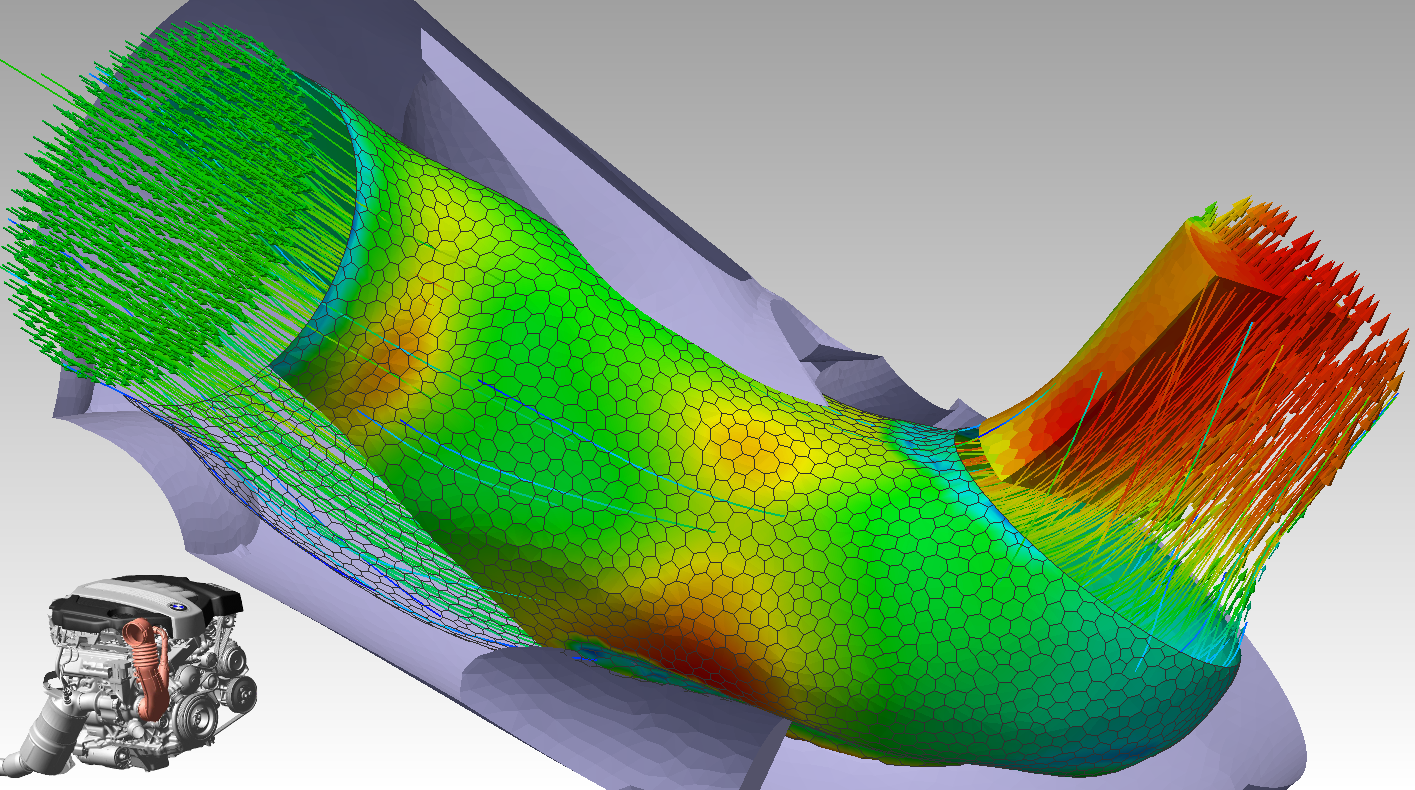
\includegraphics[width=\paperwidth,height=100pt]{FlowShapeDS4.png}%
\vbox to \paperheight{\vfil\hbox to \paperwidth{\hfil
    {\transparent{0.65}
    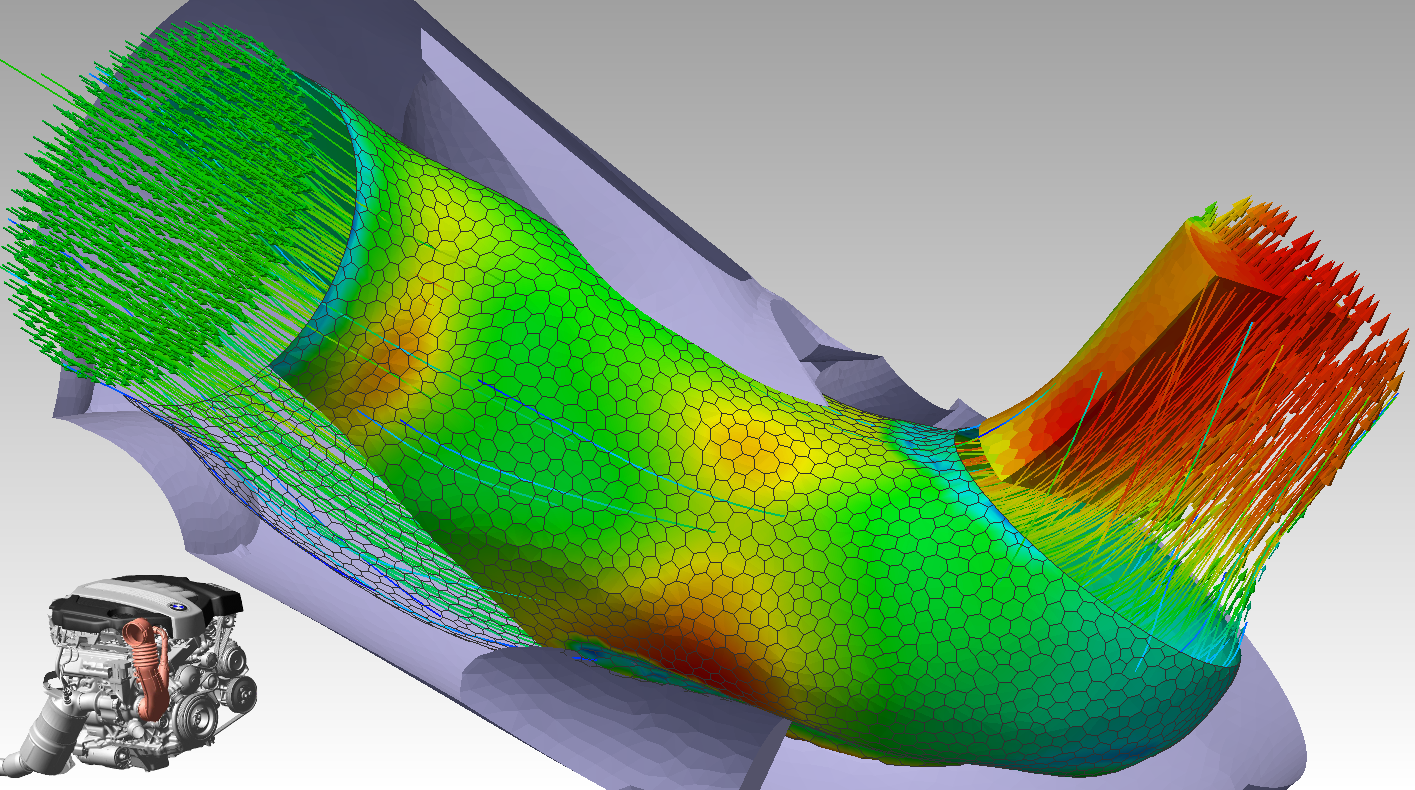
\includegraphics[width=5.1in]{FlowShapeDS4.png}}\hfil}\vfil}
}
\frame{\titlepage}
}
%
\begin{frame}
  \frametitle{Introduction of the host institute and the industrial
    partner}
  \Large{Weierstrass Institute for Applied Analysis and Stochastics}
        {\small
          \begin{minipage}{\linewidth}
            \begin{minipage}{0.725\linewidth}
              \begin{itemize}
              \item Founded in 1992
              \item project oriented research in applied mathematics
                with the aim of solving complex problems in
                technology, science and the economy.
              \item 156 employees, including 125 scientists (as at end of 2016)
              \item Scientifically independent non-university research institute
              \item Part of Forschungsverbund Berlin e.V.\, (joint
                administration for eight institutes) and a member of
                Leibniz Association
              \item Leibniz Association connects 91 research
                institutions that range in focus from the natural,
                engineering and environmental sciences via economics,
                spatial and social sciences to the humanities.
              \end{itemize}
            \end{minipage}
            \hspace{0.05\linewidth}
            \begin{minipage}{0.2\linewidth}
              
\includegraphics[scale=0.45]{wiaslogo-2010.pdf}
            \end{minipage}
          \end{minipage}
        }
\end{frame}
%
\begin{frame}
  \frametitle{Introduction of the host institute and the industrial
    partner}
  \Large{Scientific structure}
  \vspace{0.5cm}

  \begin{tabular}{cccc}
        \begin{tcolorbox}[
                    boxrule=1pt,
                    coltitle=black,
                    colframe=red!75,
                    colback=red!15!white,
                    boxsep=0pt,
                    left=4pt,right=4pt,top=2pt,bottom=2pt,
                    width=(70pt), height=(50pt),
                    adjusted title={\small RG1}]
          \tiny \centering {\sc
            Partial Differential Equations
            }
          \\ \null \vfill
          Prof. Dr. Alexander Mielke
        \end{tcolorbox}                
        &
        \begin{tcolorbox}[
                    boxrule=1pt,
                    coltitle=black,
                    colframe=green!70!blue,
                    colback=green!15!white,
                    boxsep=0pt,
                    left=4pt,right=4pt,top=2pt,bottom=2pt,
                    width=(70pt), height=(50pt),
                    adjusted title={\small RG2}]
          \tiny \centering {\sc Laser Dynamics}
          \\ \null \vfill
          PD Dr. Uwe Bandelow
        \end{tcolorbox}                
        &
        \begin{tcolorbox}[
                    boxrule=1pt,
                    coltitle=black,
                    colframe=red!70!blue,
                    colback=red!10!white,
                    boxsep=0pt,
                    left=4pt,right=4pt,top=2pt,bottom=2pt,
                    width=(70pt), height=(50pt),
                    adjusted title={\small RG3}]
          \tiny \centering
          {\sc Numerical Mathematics and Scientific Computing}
          \\ \null \vfill
          Prof. Dr. Volker John
        \end{tcolorbox}                
        &
        \begin{tcolorbox}[
                    boxrule=1pt,
                    coltitle=black,
                    colframe=yellow!70!gray,
                    colback=yellow!20!white,
                    boxsep=0pt,
                    left=4pt,right=4pt,top=2pt,bottom=2pt,
                    width=(70pt), height=50pt,
                    adjusted title={\small RG4}]
          \tiny \centering {\sc
            Nonlinear Optimization and Inverse Problems
            }
          \\ \null \vfill
          Prof. Dr. Dietmar H\"omberg
        \end{tcolorbox}                
        \\

        \begin{tcolorbox}[
                    boxrule=1pt,
                    coltitle=black,
                    colframe=pink!80!white,
                    colback=pink!20!white,
                    boxsep=0pt,
                    left=4pt,right=4pt,top=2pt,bottom=2pt,
                    width=(70pt), height=50pt,
                    adjusted title={\small RG5}]
          \tiny \centering {\sc
            Interacting Random Systems}
          \\ \null \vfill
          Prof. Dr.  Wolfgang König Partial Differential
        \end{tcolorbox}                
        &
        \begin{tcolorbox}[
                    boxrule=1pt,
                    coltitle=black,
                    colframe=blue!45!white,
                    colback=blue!15!white,
                    boxsep=0pt,
                    left=4pt,right=4pt,top=2pt,bottom=2pt,
                    width=(70pt), height=50pt,
                    adjusted title={\small RG6}]
          \tiny \centering {\sc
            Stochastic Algorithms and Nonparametric Statistics
            }
          \\ \null \vfill
          Prof. Dr.  Vladimir Spokoiny
        \end{tcolorbox}                
        &
        \begin{tcolorbox}[
                    boxrule=1pt,
                    coltitle=black,
                    colframe=green!20!gray,
                    colback=green!15!white,
                    boxsep=0pt,
                    left=4pt,right=4pt,top=2pt,bottom=2pt,
                    width=(70pt), height=50pt,
                    adjusted title={\small RG7}]
          \tiny \centering
                {\sc
                  Thermodynamic Modeling and Analysis of Phase
                  Transitions
                }
                \\ \null \vfill
          Prof. Dr. Barbara Wagner (acting head)
        \end{tcolorbox}                
        &
        \begin{tcolorbox}[
                    boxrule=1pt,
                    coltitle=black,
                    colframe=orange!50!white,
                    colback=orange!15!white,
                    boxsep=0pt,
                    left=4pt,right=4pt,top=2pt,bottom=2pt,
                    width=(70pt), height=50pt,
                    adjusted title={\small RG8}]
          \tiny \centering {\sc
            Nonsmooth Variational Problems and Operator Equations
            }
          \\ \null \vfill 
          Prof. Dr. Michael Hinterm\"uller
        \end{tcolorbox}                
  \end{tabular}
  {\footnotesize
    and three flexible research platforms
    \begin{itemize}
    \item {\bf Weierstrass Group:} Modeling, Analysis, and Scaling Limits
      for Bulk-Interface Processes (until 07/20)
      \\Dr. Marita Thomas
    \item {\bf Leibniz Group:} Probabilistic Methods for Mobile Ad-hoc Networks (until 12/17)
      \\Prof. Dr. Wolfgang König
    \item {\bf Fokus Platform:} Quantitative Analysis of Stochastic and Rough
      Systems
      \\Prof.\, Dr.\, Peter K. Friz and Dr.\, Christian Bayer
    \end{itemize}
  }
\end{frame}
%
\begin{frame}
  \frametitle{Introduction of the host institute and the industrial
    partner}
  \begin{minipage}{\linewidth}
    \begin{minipage}{0.725\linewidth}
      \Large{MATH+TEC}
            {\small
              \begin{itemize}
              \item Established in 2009
              \item Expertise in warehouse logistics, production logistics,
                transport logistics and industry optimization as well as numerical
                simulation of fluids
              \item Main products:
                \begin{enumerate}
                \item MATH.TOUR (mathematical route optimisation)
                \item MATH.PICK (warehouse optimisation software)
                \item MATH.PACK (3D packing calculation for load carriers)
                \end{enumerate}
              \end{itemize}
            }
    \end{minipage}
    \hspace{0.5cm}
    \begin{minipage}{0.2\linewidth}
      
\includegraphics[scale=0.25]{logoMathTec.png}
    \end{minipage}
  \end{minipage}
\end{frame}
%
\begin{frame}
  \centering
  \Huge Shape optimization of air ducts
\end{frame}
\frame{\frametitle{Navier-Stokes equations}
\begin{columns}[c]
\column[c]{5cm}
Stationary regime for the velocity $\buu$ and the kinematic pressure $p$:\\
$ $\\
\begin{eqnarray*}
%\label{pde_1} \nabla \cdot \left(\buu \buu^{T} \right) -\nu \Delta \buu+ \nabla p &=& \bzz  \quad in \; \Om, \\
\label{pde_1} \left( \buu \cdot \nabla \right) \buu -\nu \Delta \buu+ \nabla p &=& \bzz  \quad in \; \Om, \\
\label{pde_2} \nabla \cdot \buu &=& 0 \quad in \; \Om,\\
\label{pde_3} \buu &=& \bgg \quad on \; \Gamma_i,\\
\label{pde_4} \buu &=& \bzz \quad on \; \Gamma_w,\\
\label{pde_5} -\nu \partial_n \buu + p \bnn &=& \bzz \quad on \; \Gamma_o.
\end{eqnarray*}
%
$ $\\
\begin{eqnarray*}
%&g \; ... \text{inflow profile}\\
& \bgg:&\text{inflow profile}\\
&\nu \;:&\text{kinematic viscosity}\\
&\bnn \;:&\text{outer normal vector}\\
\end{eqnarray*}
%
\column{5cm}
\begin{figure}[htbp]
    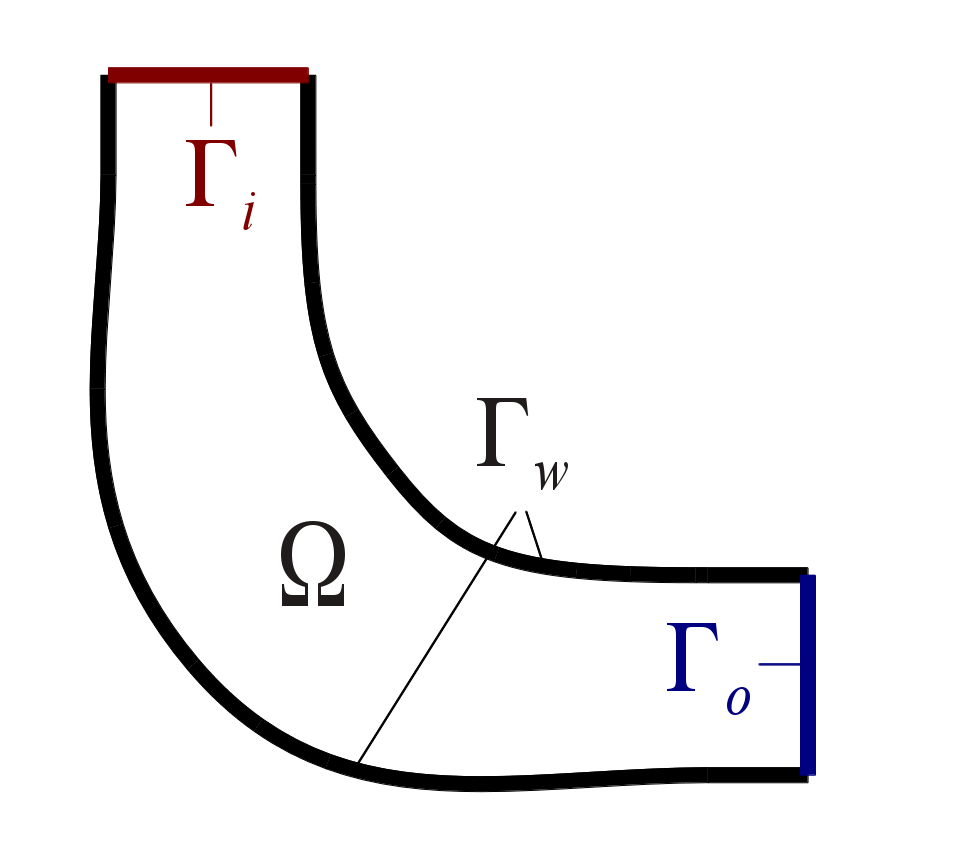
\includegraphics[scale=0.35]{geometrie_skizze_simple.png}
\end{figure}
\begin{figure}[htbp]
    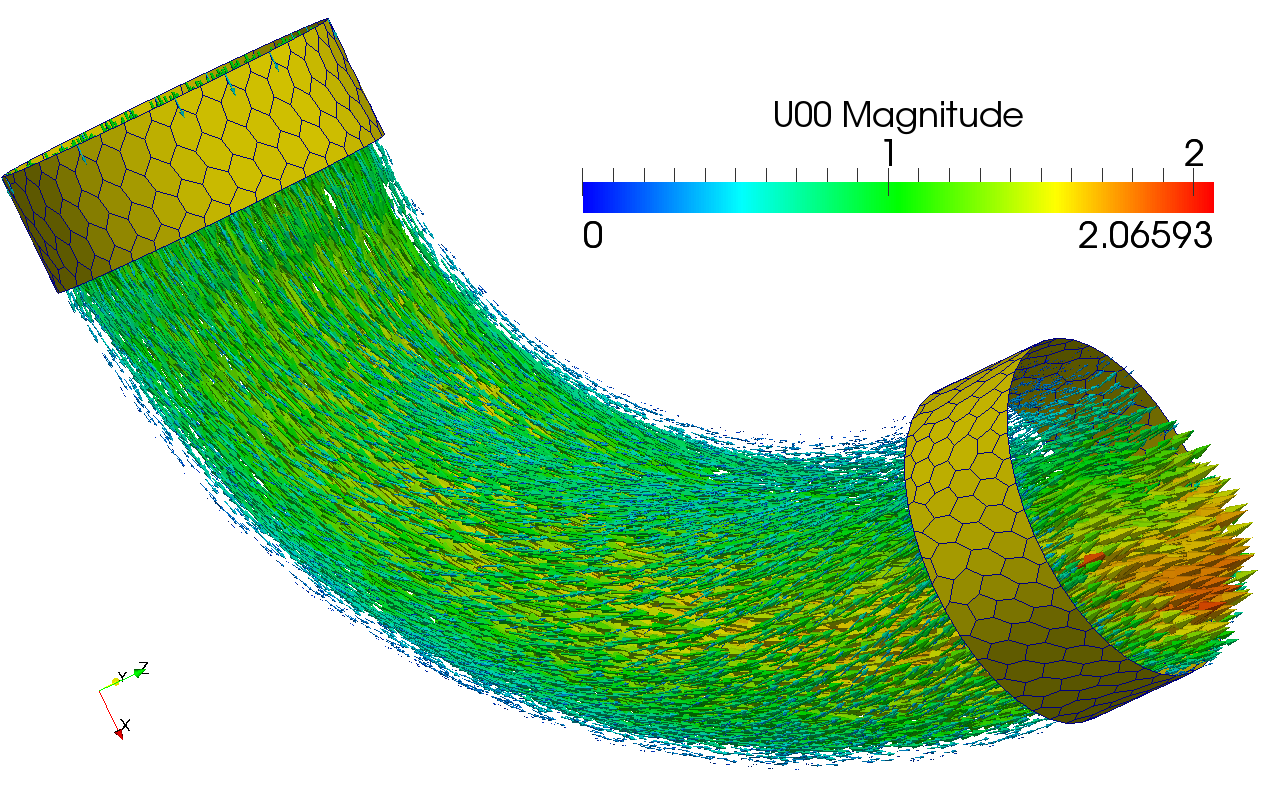
\includegraphics[scale=0.1]{TorusPrimal150.png}
%\caption{Solution $\buu$.}
\end{figure}
\end{columns}
}
%\frame{ \frametitle{Streamline profile of $\buu$ and velocity at the outlet}
%\begin{figure}[htbp]
% % \centering
%  \begin{minipage}[b]{5.5 cm}
%    \includegraphics[scale=0.13]{BMWstokesUstream.png}
%  \end{minipage}
%  \begin{minipage}[b]{5 cm}
%    \includegraphics[scale=0.13]{BMW4e4Ustream.png}
%  \end{minipage}
%  \begin{minipage}[b]{5.5 cm}
%   \includegraphics[scale=0.1]{BMWstokesU.png} 
%  \end{minipage}
%  \begin{minipage}[b]{4 cm}
%    \includegraphics[scale=0.1]{BMW4e4U.png}
%  \end{minipage}
%  \caption{Left: Stokes equations, right Navier-Stokes equations with Re=400.}
%  \label{BMWUstream}
%\end{figure}
%}


\frame{\frametitle{Uniform outflow / total pressure loss}
%Die gleichmäßige Ausströmung wird durch die Zielfunktion
To achieve \textcolor{dred}{\textbf{uniform outflow}} at the outlet the cost functional
\begin{equation}
\label{1.1} \JJ_1 \left( \buu \left( \Om \right) \right) = \frac{1}{2} \int_{\Gamma_o} \left( \buu \cdot \bnn - \bu \right)^2 \qquad \mbox{mit} \quad \bu = \frac{1}{\left| \Gamma_o \right|} \int_{\Gamma_i} -\bgg \cdot \bnn.
\end{equation}
is used.
To minimize the \textcolor{dblue}{\textbf{total pressure loss}} we use
\begin{equation}
\label{1.2} \JJ_2 \left( \buu \left( \Om \right) \right) =-\frac{|\Gamma_i|}{|\Gamma_i^\e|}\int_{\Gamma_i^\e}\left(p+\frac{1}{2}|\buu|^2\right)\buu\cdot \bnn - \frac{|\Gamma_o|}{|\Gamma_o^\e|}\int_{\Gamma_o^\e}\left(p+\frac{1}{2}|\buu|^2\right)\buu\cdot \bnn.
\end{equation}
\begin{columns}[c]
\column[c]{7cm}
\textbf{Mixed} cost functional
 \begin{equation}
\label{2.1} \JJ_{12}\left( \buu \left( \Om \right) \right)  = \left(1-\gamma \right)\JJ_1 \left( \buu \left( \Om \right) \right) + \gamma \rho \JJ_2 \left( \buu \left( \Om \right) \right)
\end{equation}
with weighting parameter $ \gamma \in \left[0,1\right]$ and 
\begin{equation*}
 \quad \rho = \begin{cases}
        \frac{\left\Vert\partial \JJ_1 \left(\buu \left( \Om^0 \right) \right) \right\Vert_{L^2\left(\Gamma_w^0\right)}}{\left\Vert\partial \JJ_2\left(\buu \left(\Om^0 \right) \right) \right\Vert_{L^2\left(\Gamma_w^0\right)}} & , \mbox{if } \gamma \in \left(0,1\right),\\ 
        1 & , \mbox{if } \gamma \in \{ 0, 1 \}.
       \end{cases}
\end{equation*}
\column{3cm}
\begin{figure}[htbp]
    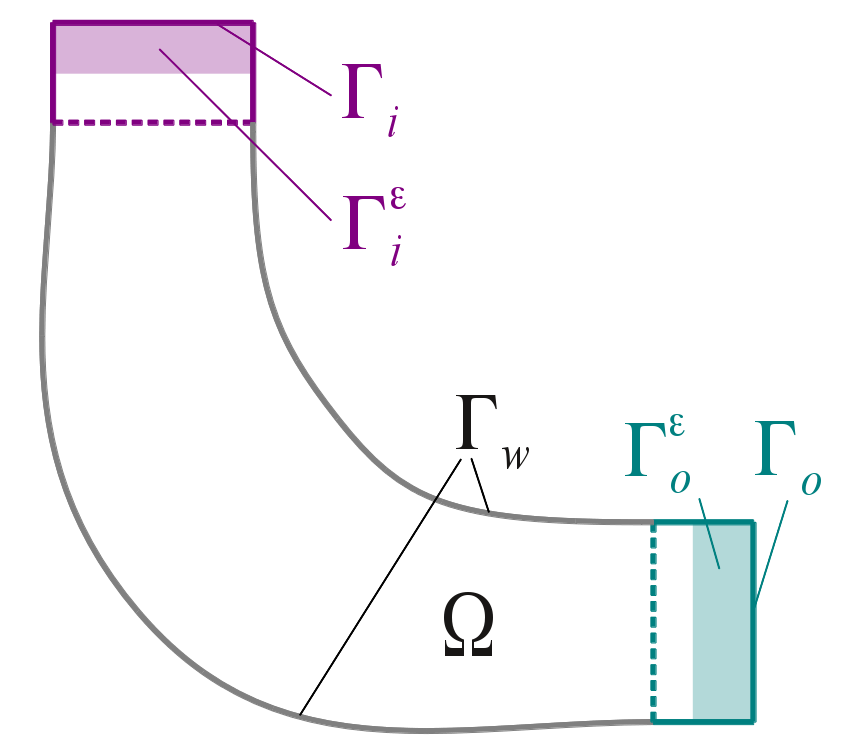
\includegraphics[scale=0.4]{geometrie_skizze_simple3.png}
\end{figure}
$ $\\
$ $\\
\end{columns}
}
%
\frame{\frametitle{Weighted shape gradient}
Adjoint equation:
%Wir wählen den adjungierten Zustand und Druck $\left( \bvv, q \right)$ als Lösung von
\begin{eqnarray*}
\label{adj_j2_1} -\nu \Delta \bvv - \left(\nabla \bvv \right)^T \cdot \buu - \nabla \bvv \cdot \buu + \nabla q &=& \textcolor{dblue}{ \gamma \; \nu k_\e\left[(\buu\cdot \bnn)\buu + \left(p+\frac{1}{2}|\buu|^2\right) \bnn\right]} \; \mbox{in} \, \Om, \\
\label{adj_j2_2} \nabla \cdot \bvv &=& \textcolor{dblue}{- \gamma\nu k_\e \buu\cdot \bnn} \quad \mbox{in} \; \Om,\\
\label{adj_j2_3} \bvv&=&0 \quad \mbox{auf} \; \Gamma_i \cup \Gamma_w, \qquad \\
\label{adj_j2_4} -\nu \partial_n \bvv - \bnn \left( \buu \cdot \bvv \right) - \left( \buu \cdot \bnn \right) \bvv  + q \bnn 
&=&\textcolor{dred}{ - \left(1-\gamma\right) \nu \left(\buu \cdot \bnn - \bu\right) \bnn}\quad \mbox{auf}\; \Gamma_o
%&=& -\frac{1}{\nu} \left( \bnn \left( \buu \cdot \bvv \right) + \left( \buu \cdot \bnn \right) \bvv  - q \bnn \right) \quad \mbox{auf}\; \Gamma_o \qquad \quad
\end{eqnarray*}
with
\begin{minipage}[b]{5.3 cm}
\begin{equation*}
k_\e\left(x\right) = \begin{cases}
        -\frac{|\Gamma_i|}{|\Gamma_i^\e|} & \mbox{if } x \in \Gamma_i^\e, \\
        -\frac{|\Gamma_o|}{|\Gamma_o^\e|} & \mbox{if } x \in \Gamma_o^\e, \\
        0 & \mbox{else}.
       \end{cases}
\end{equation*}
\end{minipage}
%\begin{minipage}[b]{4.6 cm}
%und Gewichtungsparametern \textcolor{blue}{$\rho_{\Omega}$}, \textcolor{red}{$\rho_{\Gamma}$}.
%\end{minipage}
$ $\\
$ $\\
%
\noindent\rule{11cm}{0.4pt}
\begin{minipage}[b]{5.5 cm}
$ $\\\\
Euler-semiderivative:\\
\begin{equation*}
\label{fg_2_0}\partial \JJ_{12}^\gamma\left(\Om;V\right) = \int_{\Gamma_w} \left[ \partial_n \bvv \cdot \partial_n \buu \right] V \cdot \bnn. \qquad \qquad \quad
\end{equation*}
\end{minipage}
\begin{minipage}[b]{4.7 cm}
$ $\\\\
Shape gradient:\\
\begin{equation*}
\label{fg_1} D \JJ_{12}^\gamma \left(\Om \right) = \left( \partial_n \bvv \cdot \partial_n \buu \right) \arrowvert_{\Gamma_w}. \qquad \qquad \quad
\end{equation*}
\end{minipage}
}
\frame{\frametitle{Adjoint solution and shape gradient}
\begin{columns}[c]
\column[c]{5.5cm}
Shape gradient on a simple 3D geometry with Reynolds number 150:\\
$ $\\ 
The solution $\buu$ of the Navier-Stokes equations is shown in the upper right figure.\\
$ $\\
The corresponding adjoint solution and the \textbf{negative shape gradient} coloured on the surface are presented in the figures below.  
\column{5cm}
\begin{figure}[htbp]
    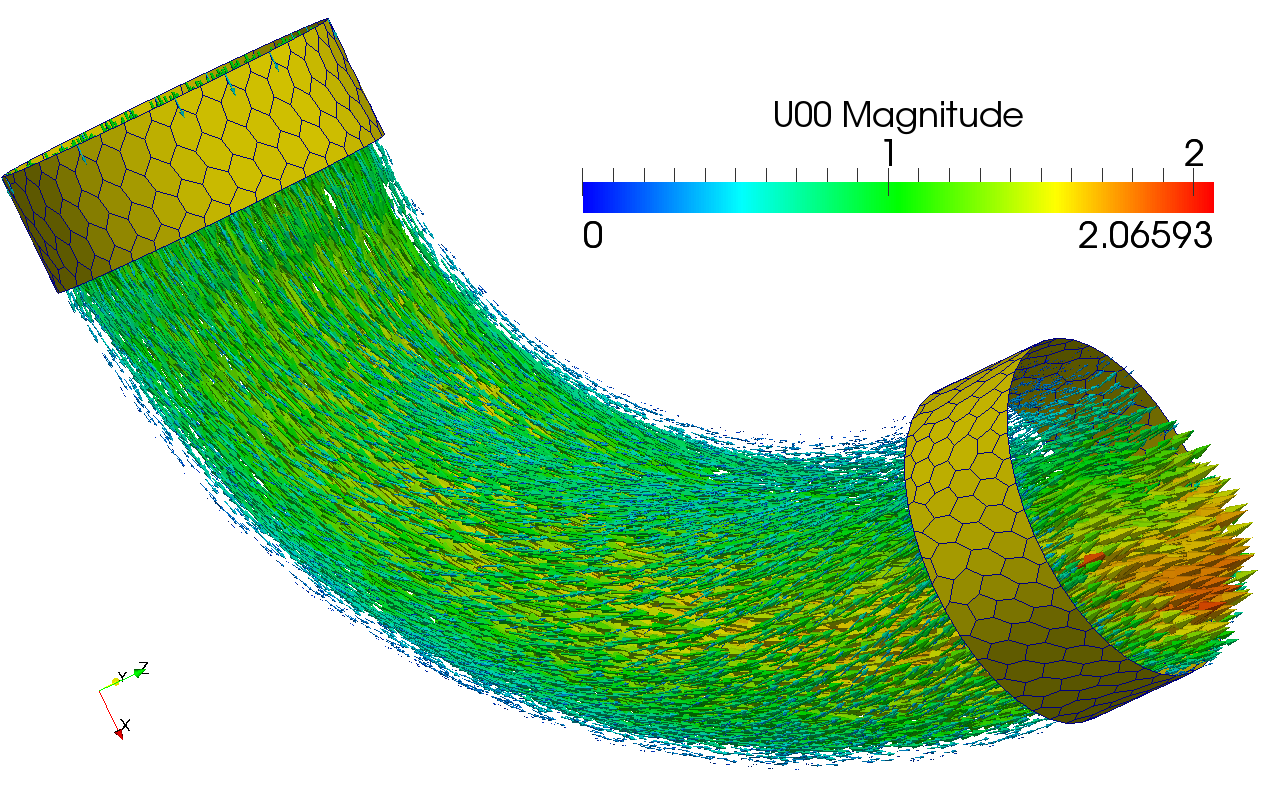
\includegraphics[scale=0.11]{TorusPrimal150.png}
%\caption{Solution $\buu$ of the Navier-Stokes equations.}
\end{figure}
\end{columns}
%
%
%
\begin{columns}[c]
\column[c]{5cm}
\begin{figure}[htbp]
    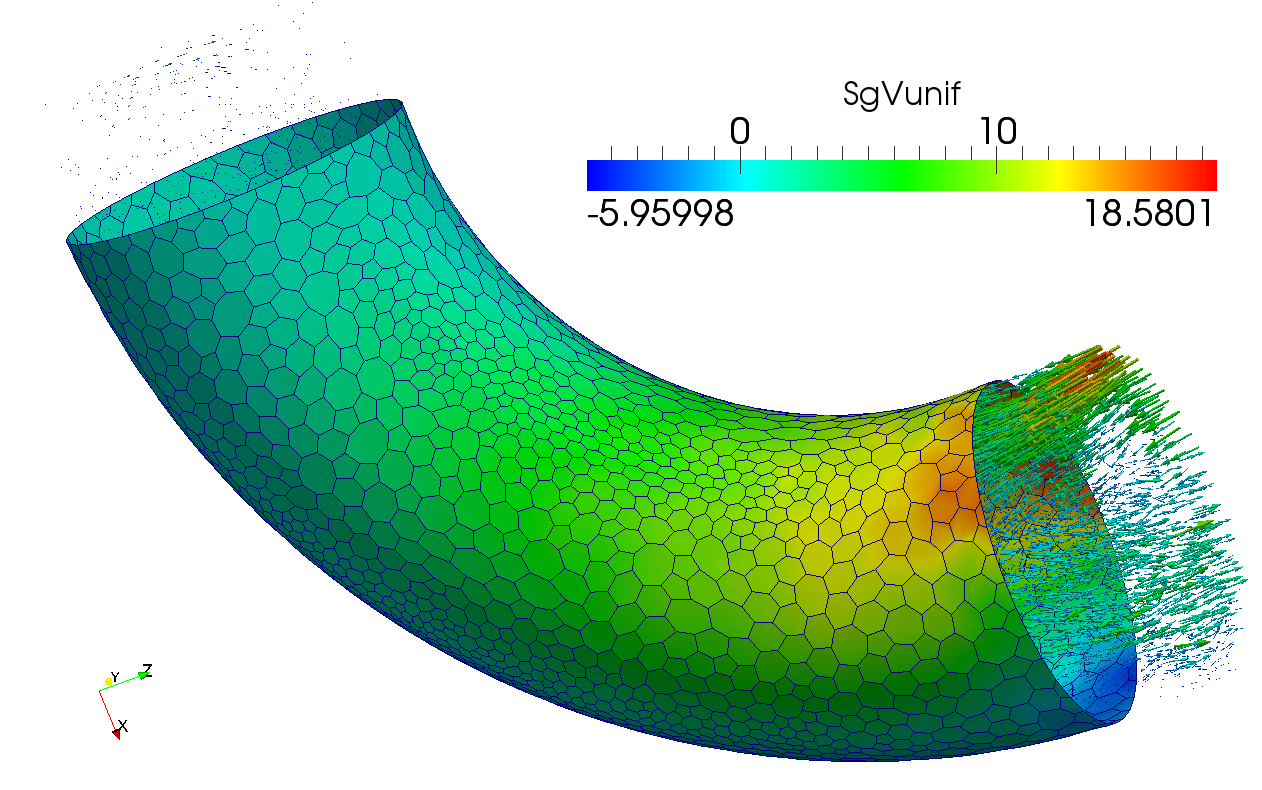
\includegraphics[scale=0.11]{TorusAdjUnif150.png}
  \caption{Uniform outflow.}
\end{figure}
\column{5cm}
\begin{figure}[htbp]
    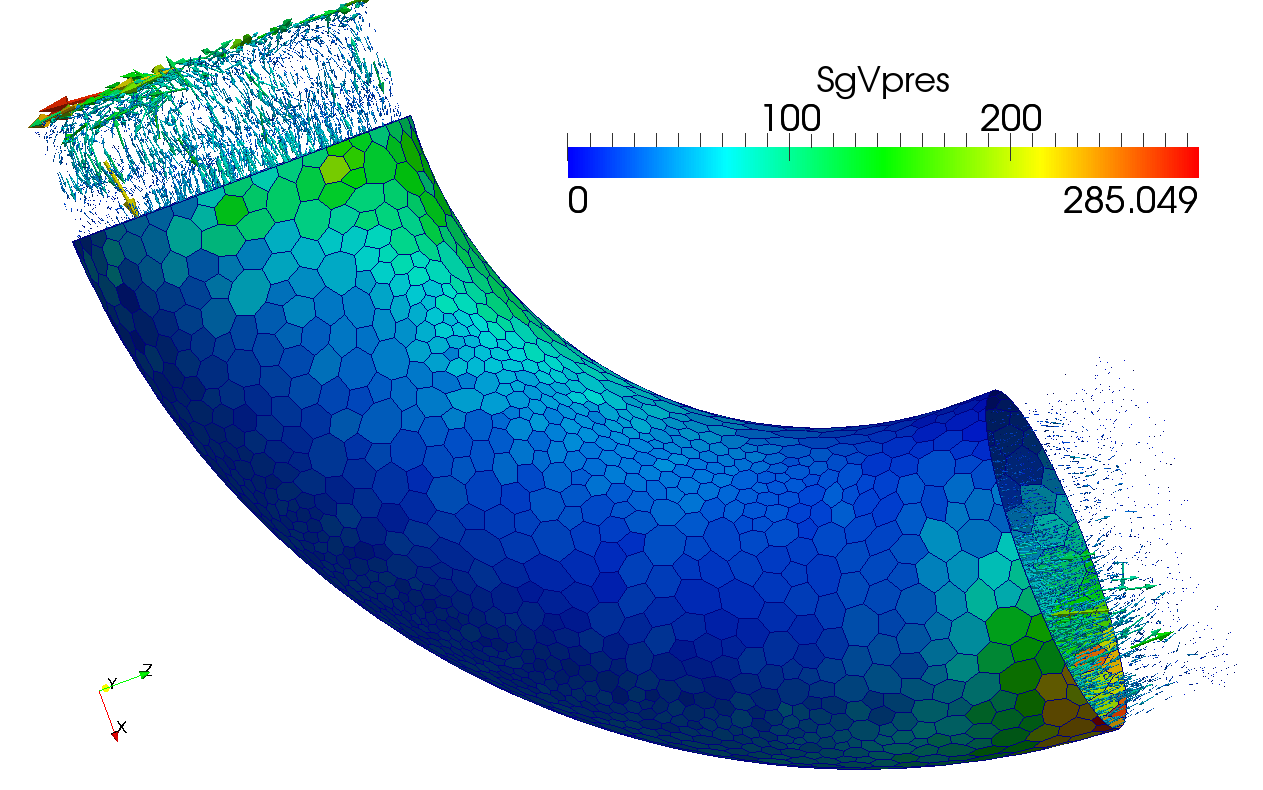
\includegraphics[scale=0.11]{TorusAdjPress150.png}
  \caption{Total pressure loss.}
\end{figure}
\end{columns}
$ $\\
$ $\\
$ $\\
$ $\\
}
%
%
\frame{\frametitle{Descent algorithm: calculation of the shape gradient}
\begin{tikzpicture}[auto]
{\footnotesize
% nodes
\node [block1] (start) 
{};
\node [block2, below of=start, node distance=2.625cm] (p0)
{\begin{itemize}
  \item Solve primal equation in $\Om^k$ $\rightarrow \left(\buu,p\right)$.
  \item Solve adjoint equation in $\Om^k$ $\rightarrow \left(\bvv,q\right)$.
  \item Calculate shape gradient: 
\begin{equation}
\nonumber \DD \JJ_{12}^\alpha \left(\Om^k;\bxx\right) 
= \partial_n \bvv\left(\Om^k;\bxx\right) \cdot \partial_n \buu\left(\Om^k;\bxx\right) 
+ \alpha \, \ell \left( \bxx \right) 
\end{equation} 
 for $\bxx$ on $\Gamma_w$.
\end{itemize}
};
\node [block, left of=start, node distance=5.6cm] (s0) 
{Initial data};
\node [block, below of=s0, node distance=1.3cm] (s1)
{Generate mesh};
\node [block, below of=s1, node distance=1.3cm] (s2)
{Calculate shape gradient};
\node [block, below of=s2, node distance=1.3cm] (s3)
{Linesearch};
\node [block, below of=s3, node distance=1.0cm] (s4)
{Move mesh};
\draw [](s2) -- (p0);
\path [line] (s0) -- (s1);
\path [line] (s1) -- (s2);
\path [line] (s2) -- (s3);
\path [line] (s4) -- (-5.6,-5.8) -- node {mesh quality } (-7.9,-5.8)  --  (-7.9,-1.3) -- node {bad} (s1);
\path [line] (-7.9,-2.6) --node {good} (s2) ;
}    
\end{tikzpicture}
}
\frame{\frametitle{Descent algorithm: usage of Armijo linesearch}
\begin{tikzpicture}[auto]
{\footnotesize
% nodes
\node [block1] (start) 
{};
\node [block2, below of=start, node distance=2.625cm] (p0)
{Armijo - linesearch:
%\textbf{Armijo - linesearch:}
\begin{equation}
\nonumber \label{armijo1}\JJ_{12}^\alpha  \left( \Om^{k+1} \right) \leq \JJ_{12}^\alpha \left( \Om^{k} \right) - \mu s_k \lVert \DD \JJ_{12}^\alpha \left( \Om^{k}  \right) \rVert_{L^2\left(\Gamma_w^k\right)} 
%\label{armijo1}\JJ_{12}^\alpha \left( \buu\left(\Om^{k+1} \right) \right) \leq \JJ_{12}^\alpha \left( \buu \left( \Om^{k} \right) \right) - \mu s_k \lvert \partial \JJ_{12}^\alpha \left( \buu \left(\Om^{k} \right); V \right) \rvert 
\end{equation}
with $0<\mu<1$ and $\Om^{k+1}=\T_{D\left(s_k, \Om^k\right)} \left(\Om^k\right)$\\ 
$ $\\
$ $\\
We need to evaluate the cost functional in $\Om_{k+1}$. This requires to solve the primal equation, therefore:
\begin{itemize}
 \item ensure mesh quality of $\Om_{k+1}$ (by reduction of the step length), 
 %\item use an efficient sequence of calculations to avoid two times calculations of the primal equation.
\item guarantee efficiency by avoiding unnecessary recalculations of the primal solution.

\end{itemize}
};
\node [block, left of=start, node distance=5.6cm] (s0) 
{Initial data};
\node [block, below of=s0, node distance=1.3cm] (s1)
{Generate mesh};
\node [block, below of=s1, node distance=1.3cm] (s2)
{Calculate shape gradient};
\node [block, below of=s2, node distance=1.3cm] (s3)
{Linesearch};
\node [block, below of=s3, node distance=1.0cm] (s4)
{Move mesh};
\draw [](s3) -- (-3.06,-3.9);
\path [line] (s0) -- (s1);
\path [line] (s1) -- (s2);
\path [line] (s2) -- (s3);
\path [line] (s4) -- (-5.6,-5.8) -- node {mesh quality } (-7.9,-5.8)  --  (-7.9,-1.3) -- node {bad} (s1);
\path [line] (-7.9,-2.6) --node {good} (s2) ;
}    
\end{tikzpicture}
}
%
%\frame{\frametitle{Descent algorithm: details}
%\begin{figure}[htbp]
%    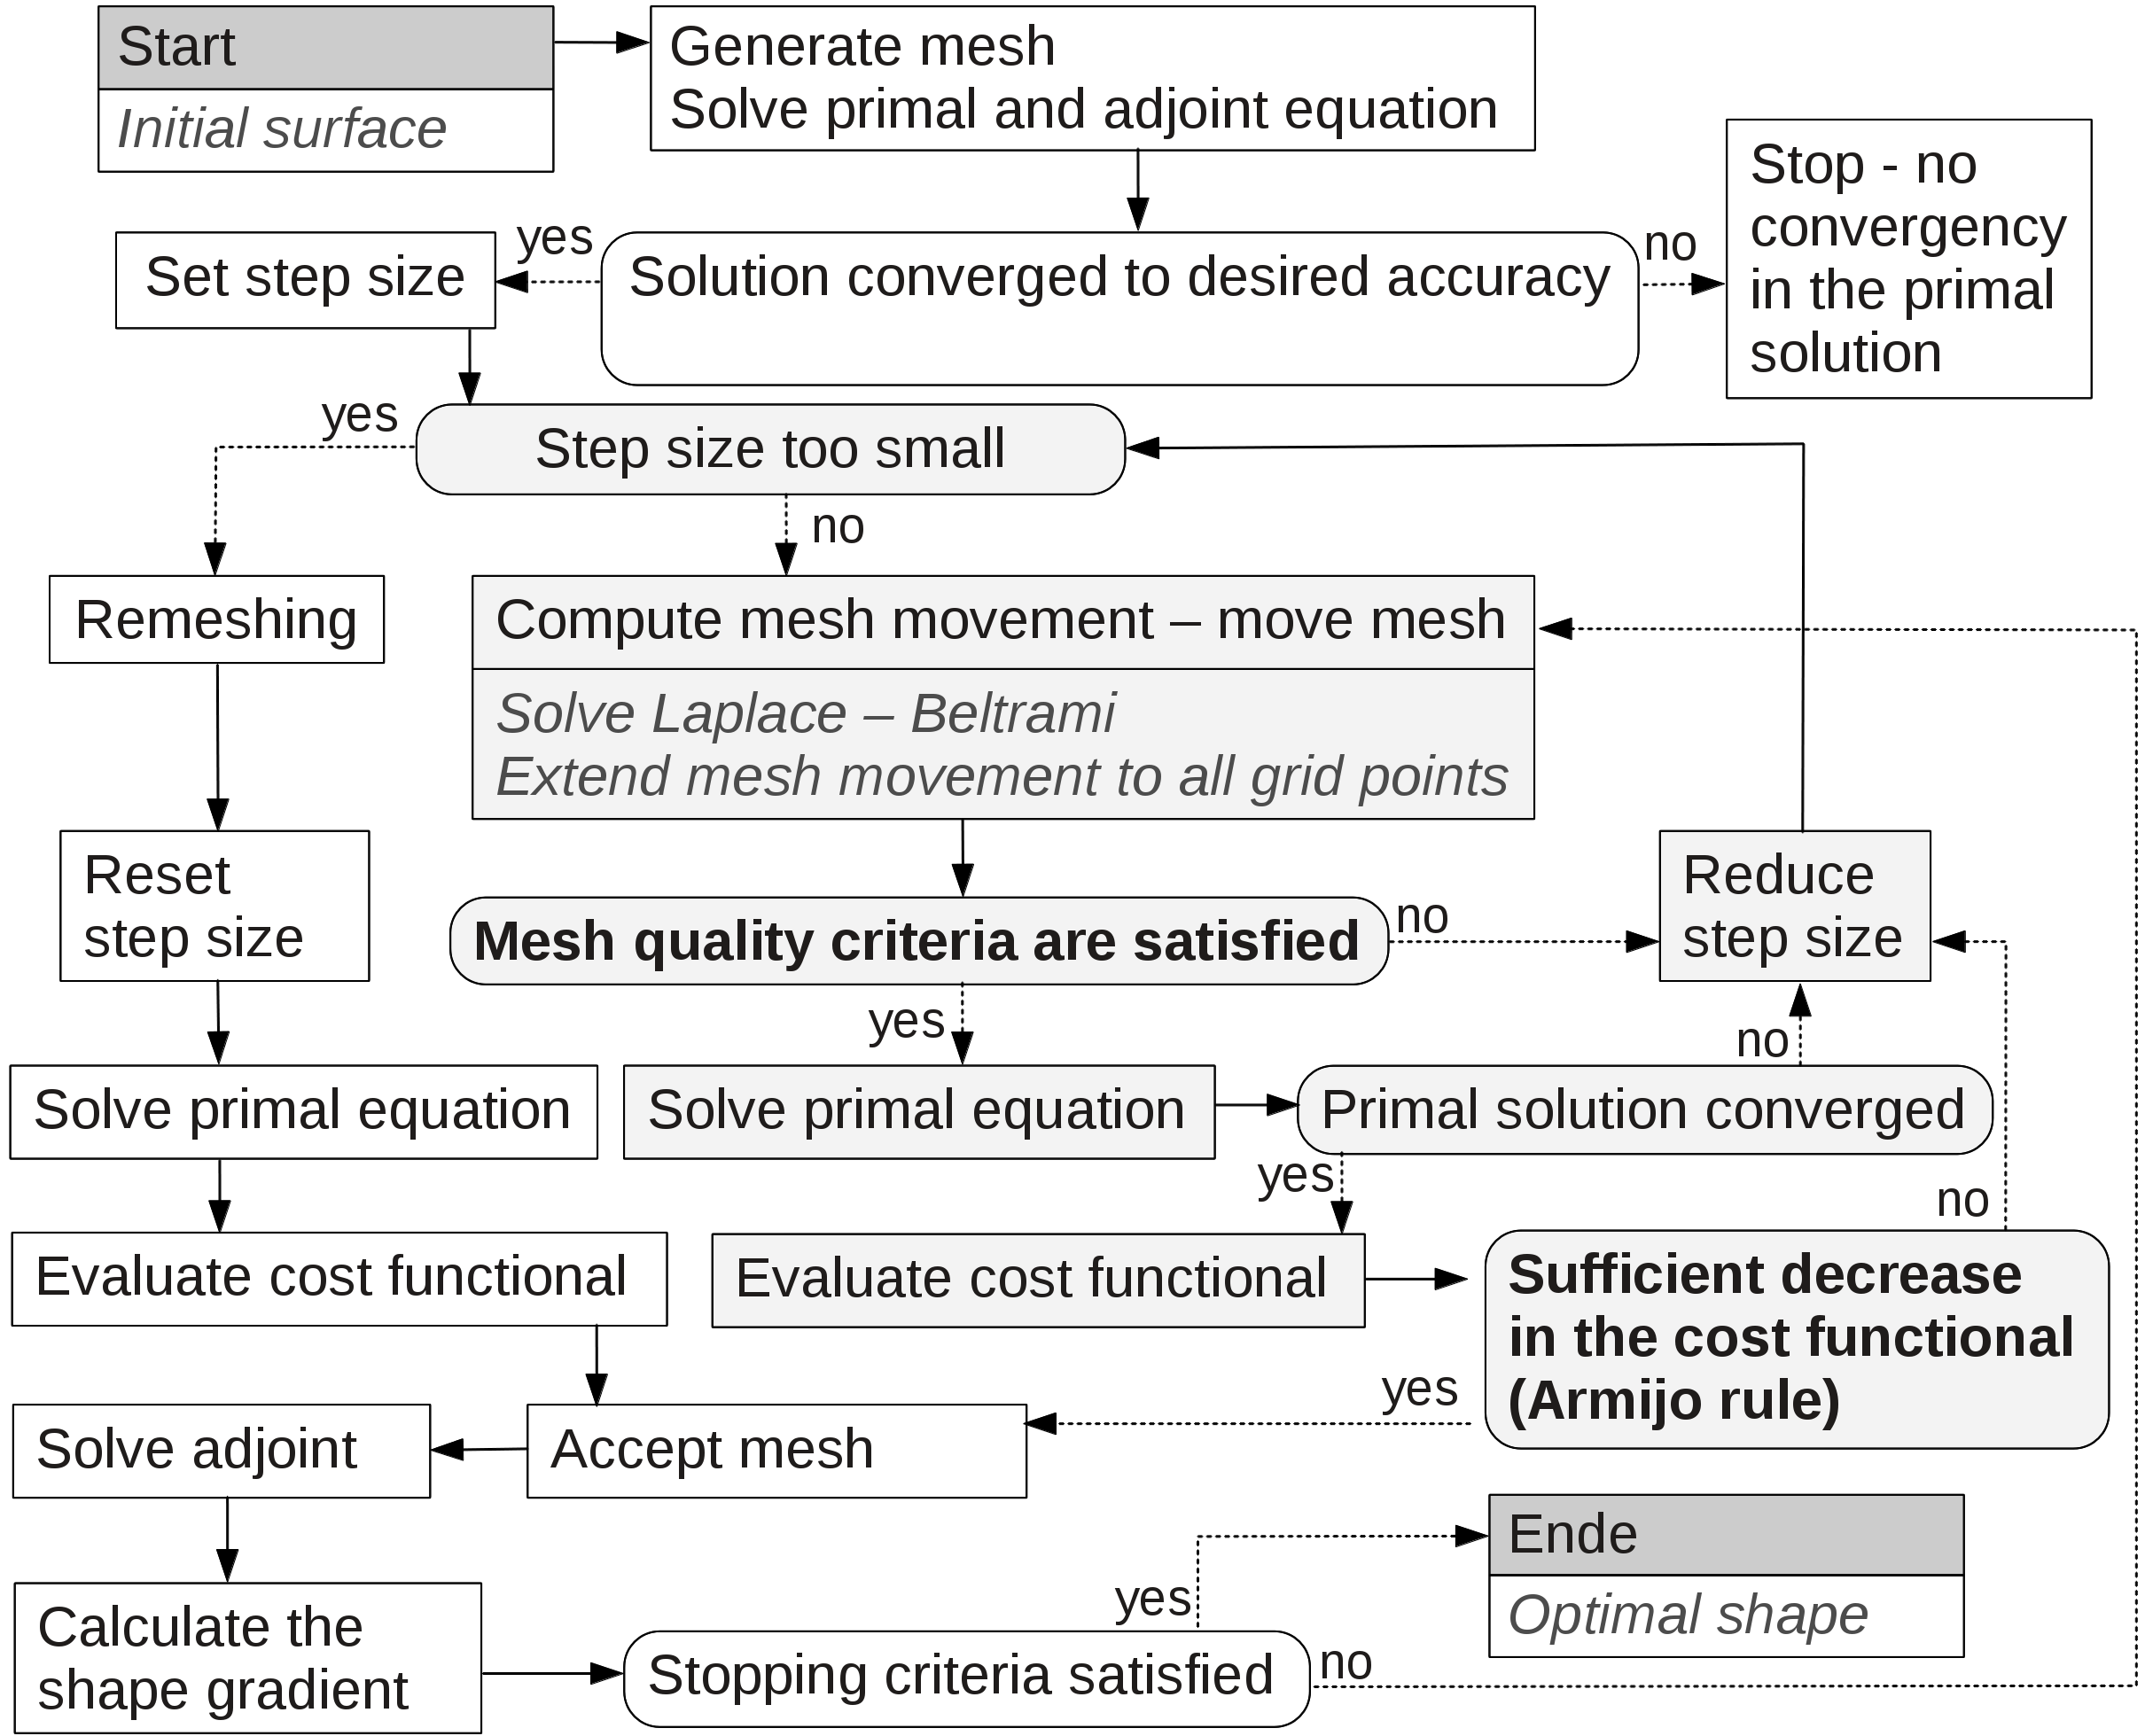
\includegraphics[scale=0.35]{struktogrammShortEngl3.png}
%  %\caption{Uniform outflow.}
%\end{figure}
%}
%
%\frame{\frametitle{Shape optimization on a simple 3D geometry}
%Considering the mixed cost funcional for Reynolds number 200 by using the Star-CD CCM+ direct numerical simulation (DNS). 
%%
%\begin{figure}[htbp]
%  \centering
%    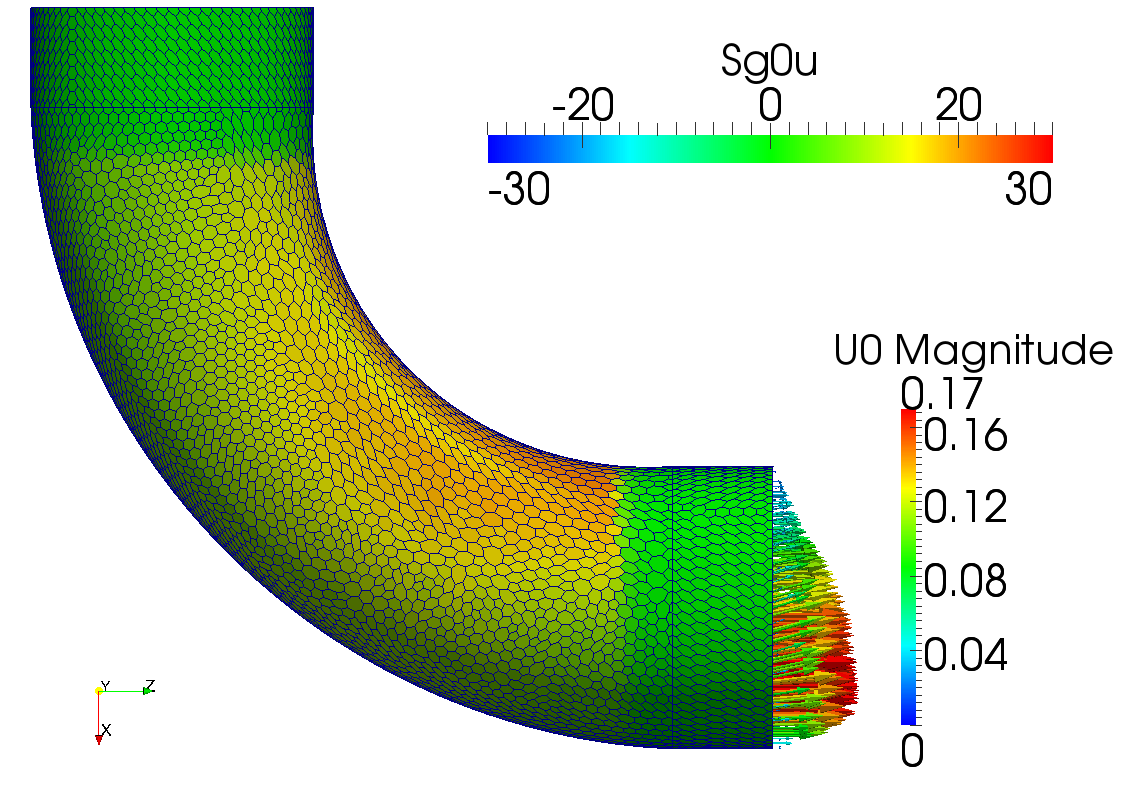
\includegraphics[scale=0.145]{TORre200_i0.png} 
%    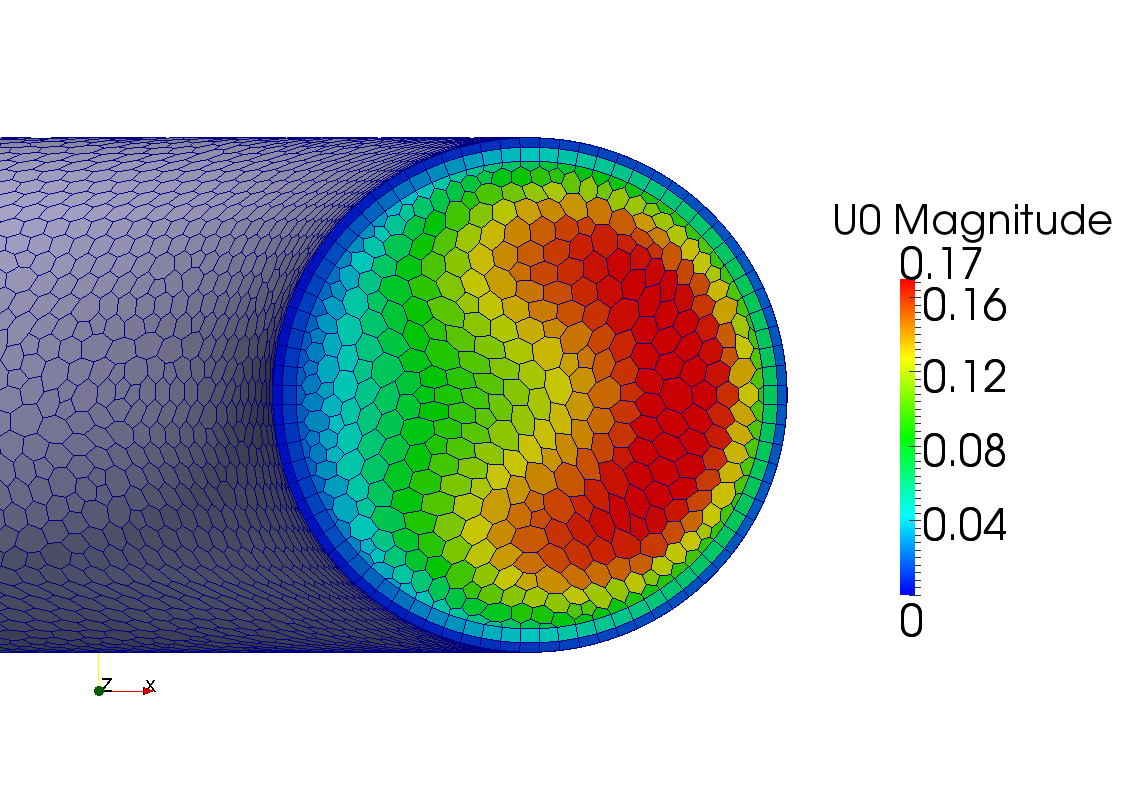
\includegraphics[scale=0.145]{TORre200_i0_out.png} 
%   \caption{
%\textcolor{white}{.} \newline
%\textbf{Left}: Negativ shape gradient on the surface and outlet velocity profile on the initial geometry.
%\newline
%\textbf{Right}: Intensity of the outlet velocity on the initial geometry.
%}
%\end{figure}
%$ $\\
%$ $\\
%$ $\\
%}
%%
%%
%\frame{\frametitle{Shape optimization on a simple 3D geometry}
%Considering the mixed cost funcional for Reynolds number 200 by using the Star-CD CCM+ direct numerical simulation (DNS). 
%%
%\begin{figure}[htbp]
%  \centering
%    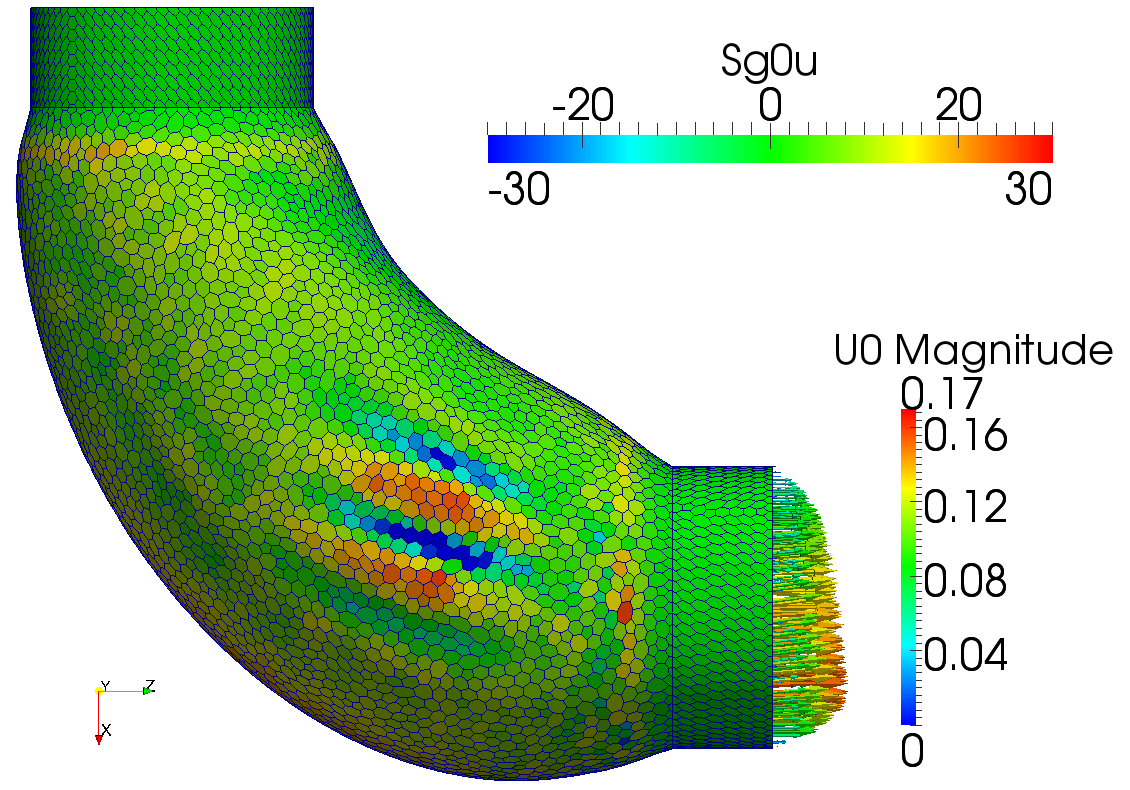
\includegraphics[scale=0.145]{TORre200_i60.png} 
%    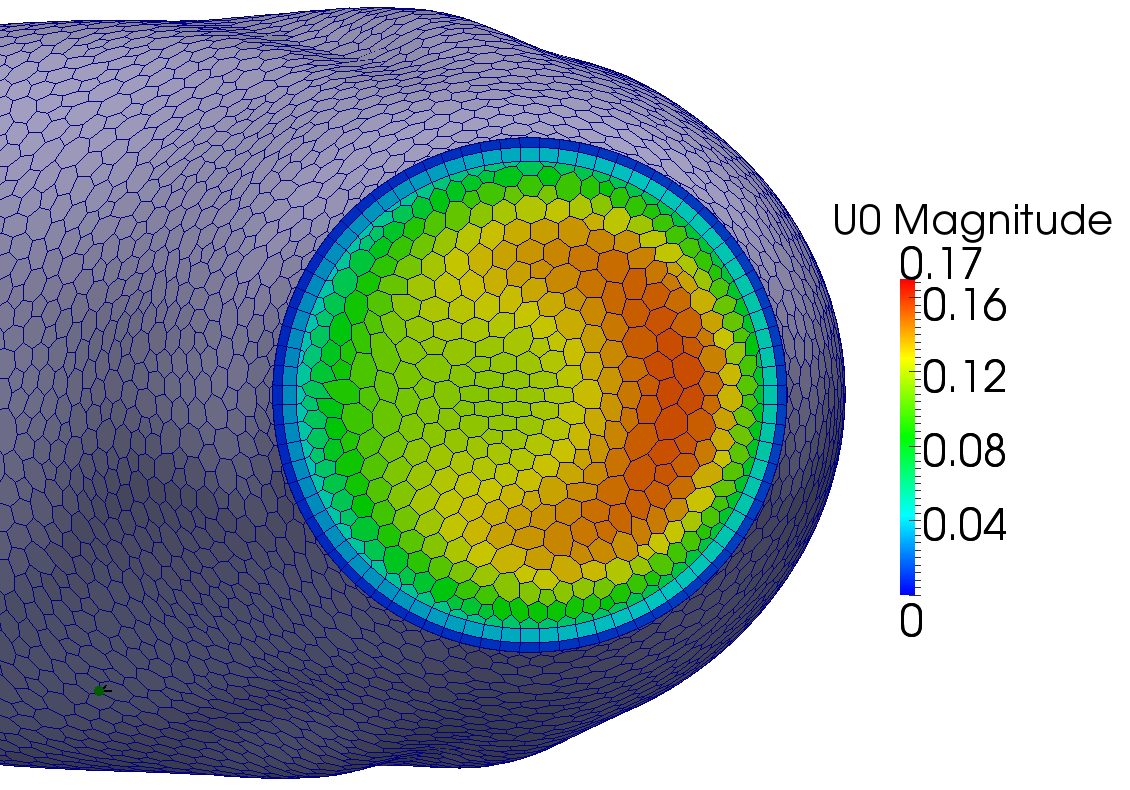
\includegraphics[scale=0.145]{TORre200_i60_out.png}   
%   \caption{
%\textcolor{white}{.} \newline
%\textbf{Left}: Negativ shape gradient on the surface and outlet velocity profile after 60 iterations.
%\newline
%\textbf{Right}: Intensity of the outlet velocity on the initial geometry after 60 iterations.
%}
%\end{figure}
%$ $\\
%$ $\\
%$ $\\
%}
%%
%%
%\frame{\frametitle{Shape optimization on a simple 3D geometry}
%Considering the mixed cost funcional for Reynolds number 200 by using the Star-CD CCM+ direct numerical simulation (DNS).
%%Testrechnung für 3D Krümmer mit Star-CD CCM+ DNS Lösereinstellungen (ohne Turbulenzmodell) mit Re=200.\\
%%Aussagekräftigere Werte im Zielfunktional - keine negativen Effekte aufgrund des Remeshings erkennbar.
%%
%\begin{figure}[htbp]
%  \centering
%    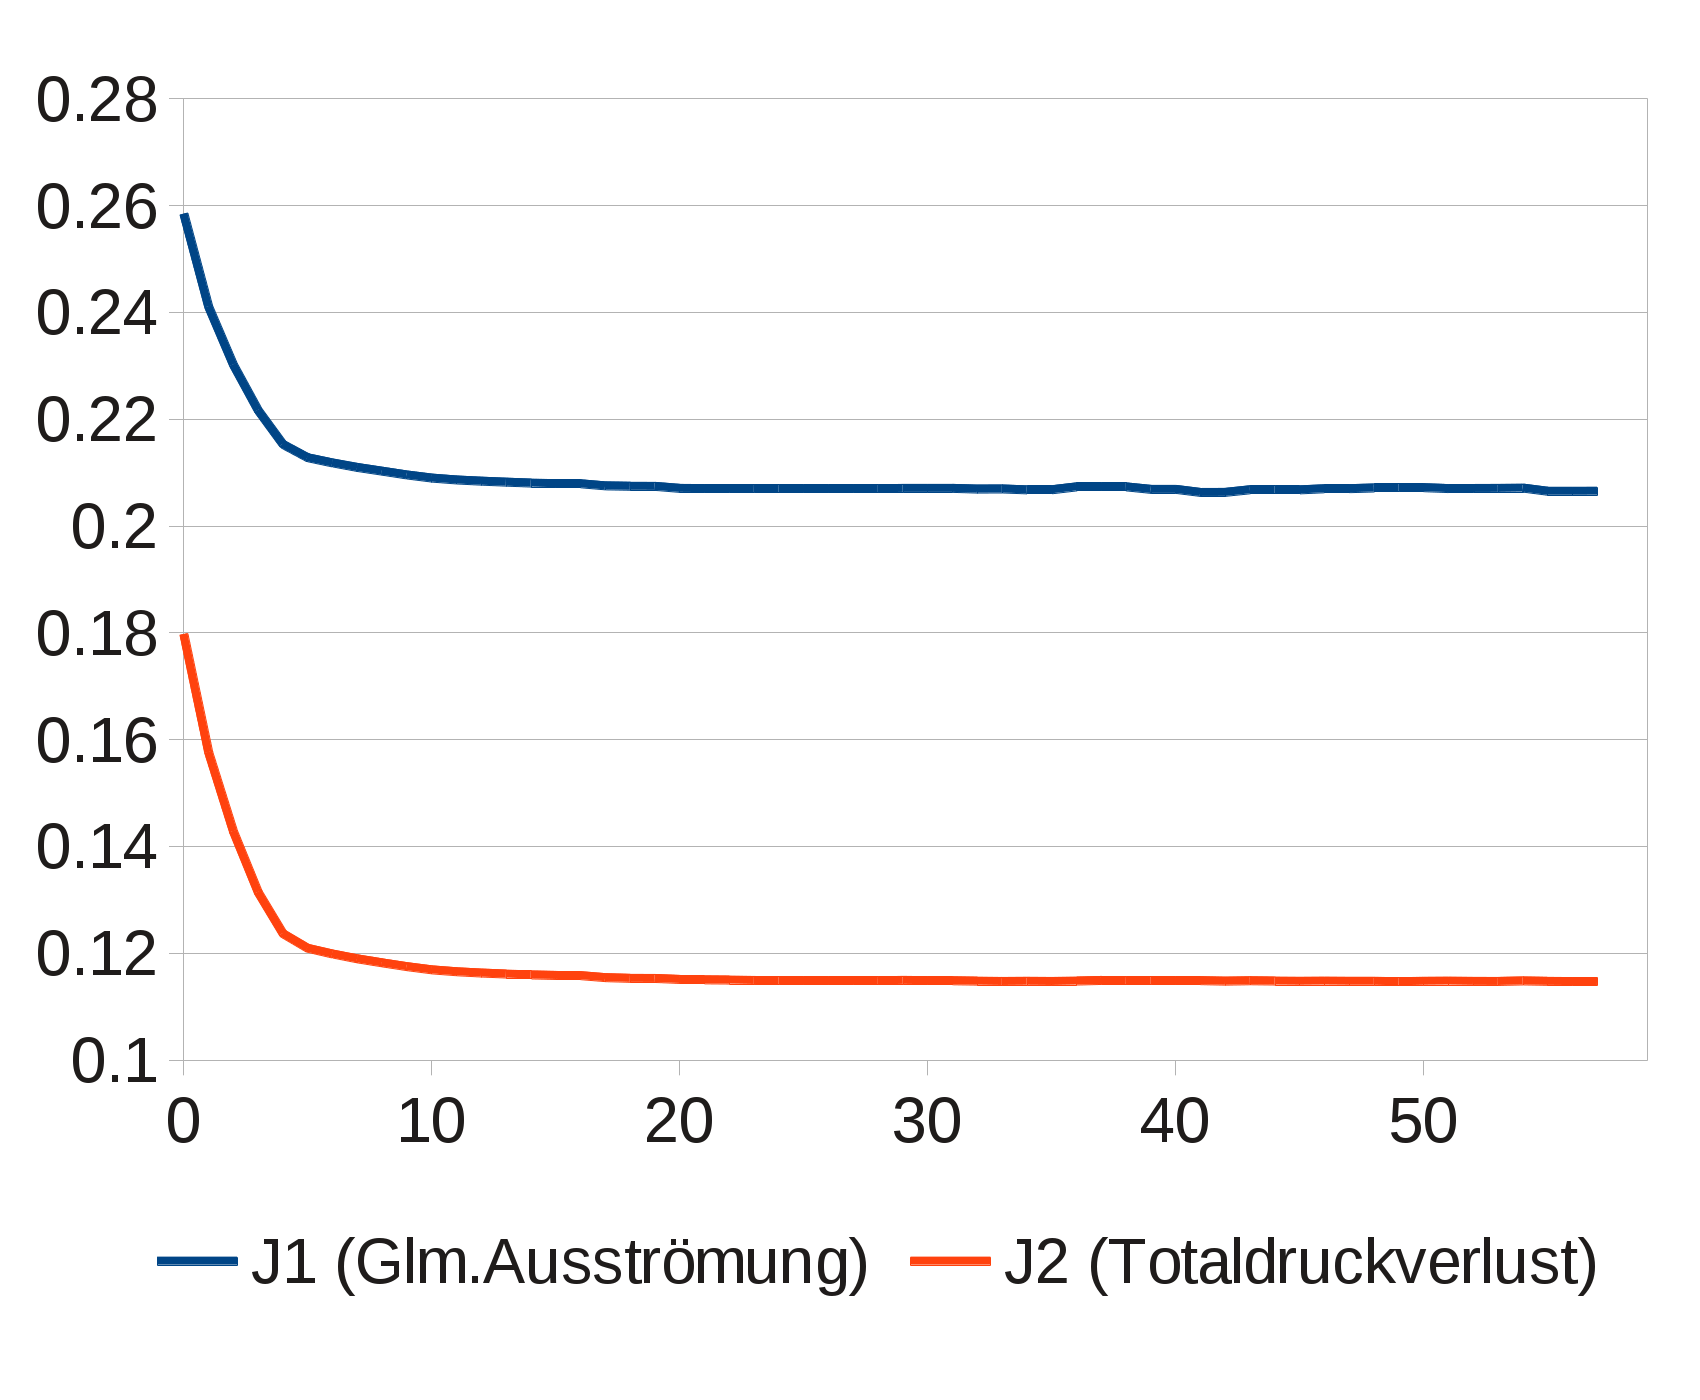
\includegraphics[scale=0.3]{fv_J1_J2_ohneVolRed.png} 
%  \caption{Values of the functionals $\JJ_1$ and $\JJ_2$,  60 iterations (20 remeshings).}
%\end{figure}
%$ $\\
%$ $\\
%$ $\\
%}
%
%
%
\frame{\frametitle{Geometrical constraint: design space}
\begin{figure}[htbp]
 % \centering
  \begin{minipage}[b]{5 cm}
    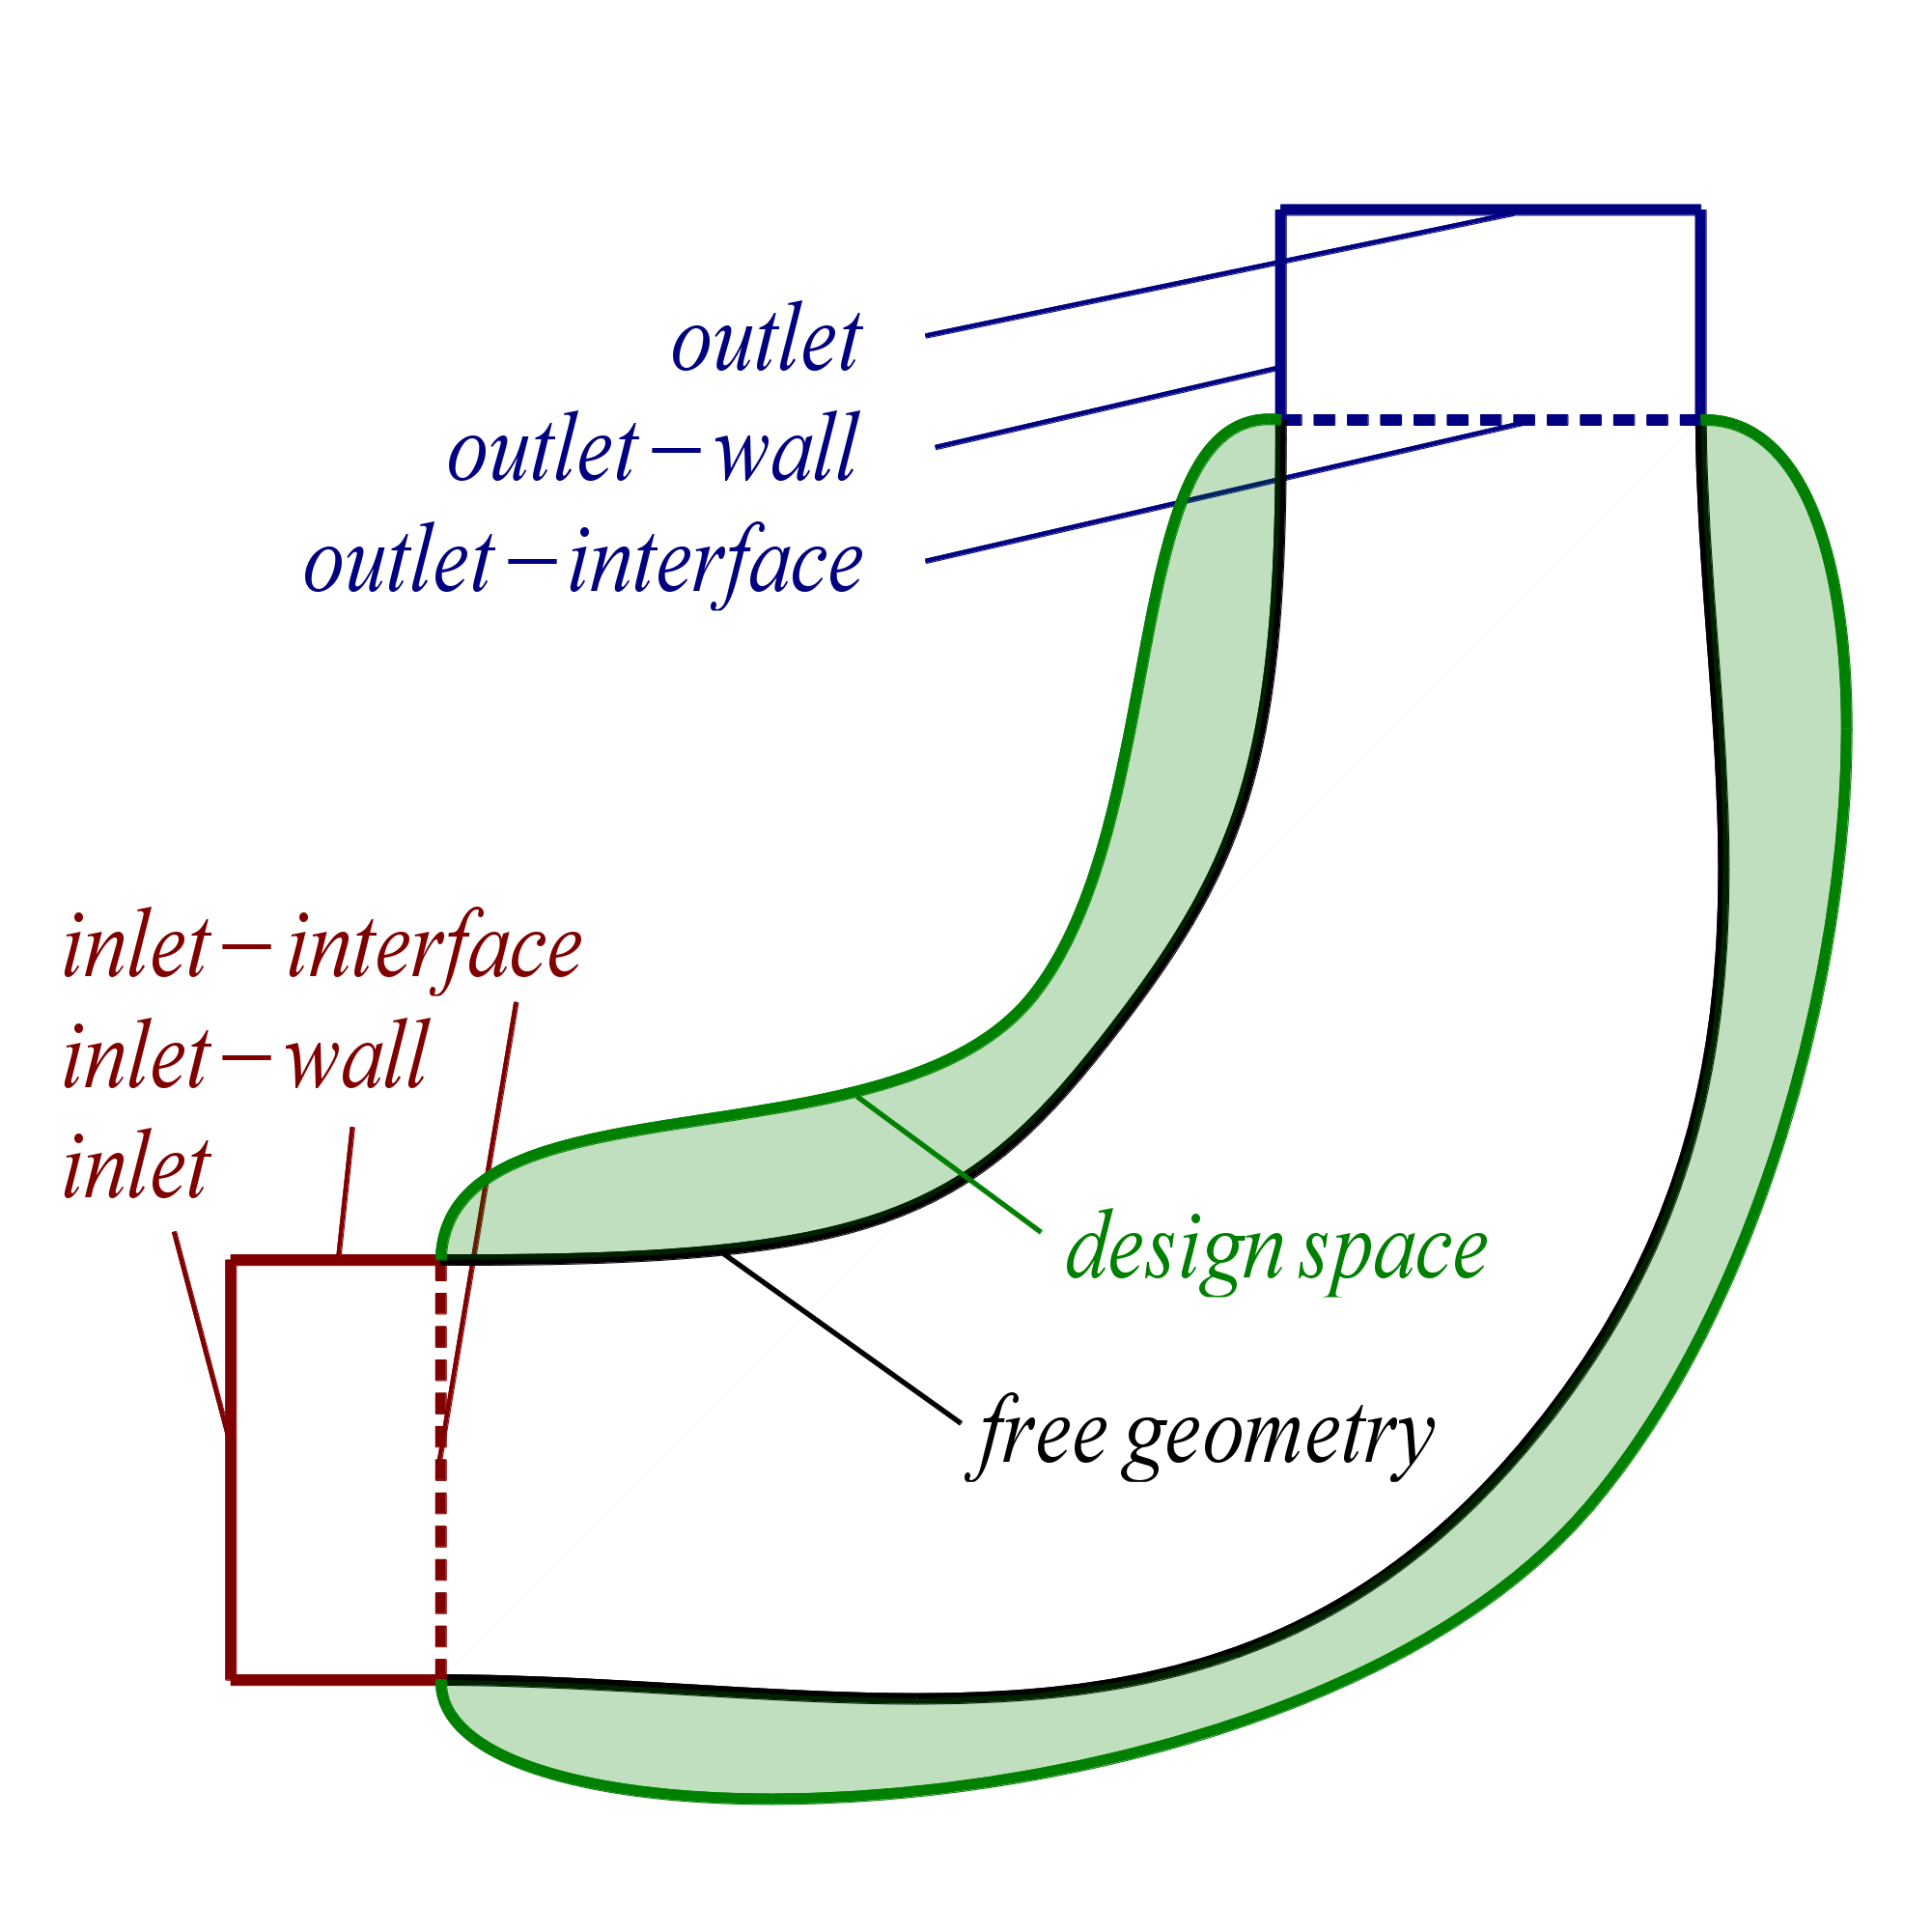
\includegraphics[scale=0.2]{geometrie_skizze_stl.png}
  \end{minipage}
  \begin{minipage}[b]{5 cm}
    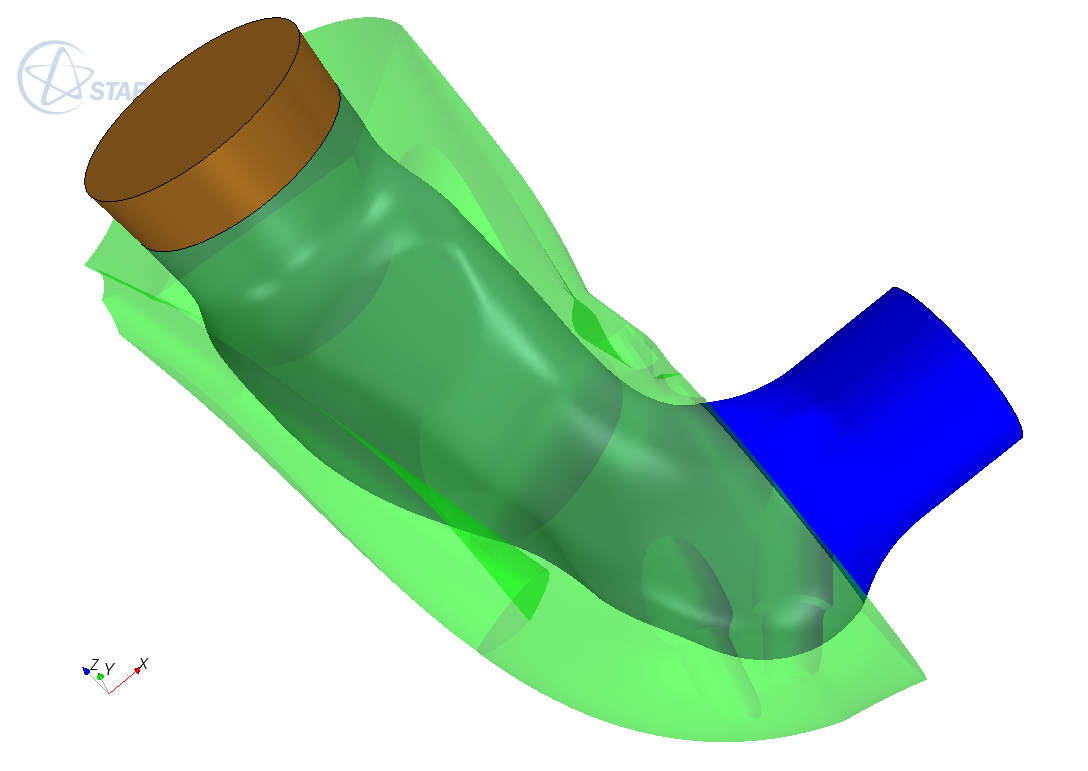
\includegraphics[scale=0.13]{darstellung_bauraum.png}
  \end{minipage}
  \begin{minipage}[b]{4 cm}
    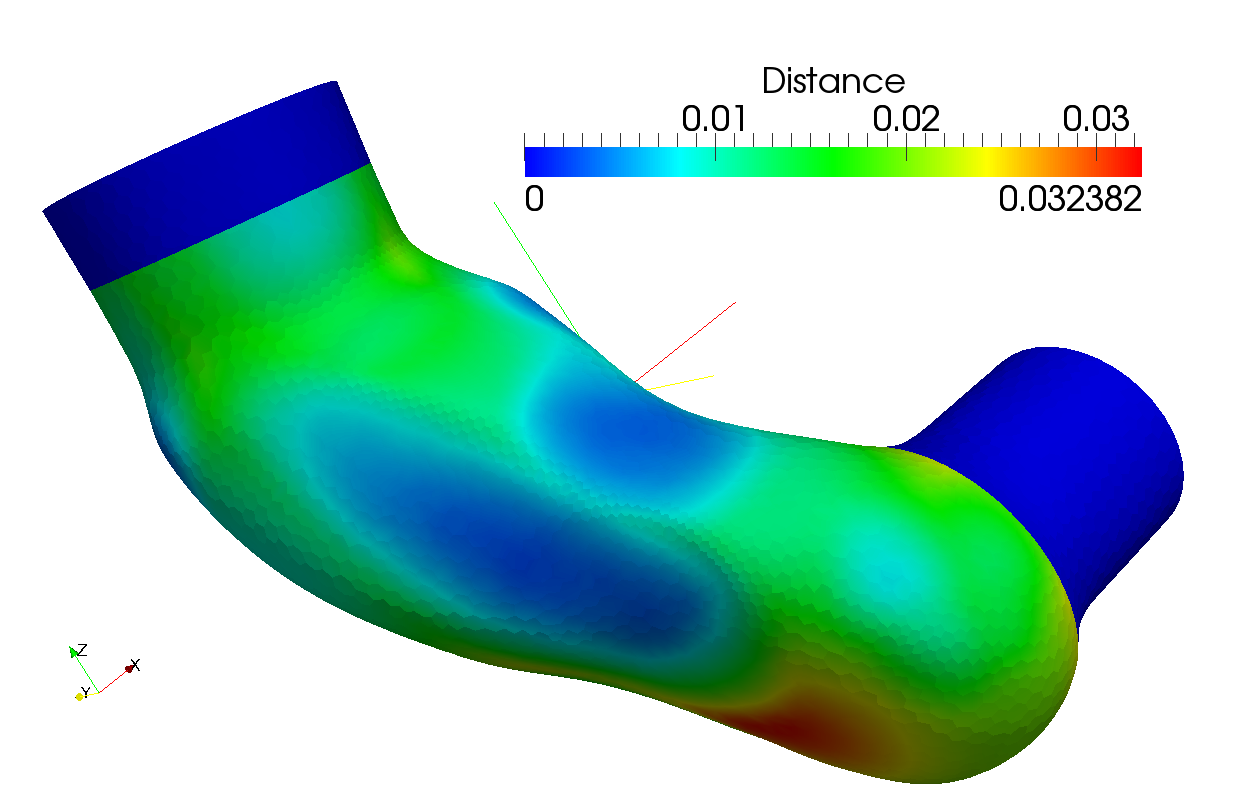
\includegraphics[scale=0.115]{distanz_bauraum.png}
  \end{minipage}
  \caption{Sketch, geometry with transparent design space, \newline \textcolor{white}{.} \qquad \quad \;  geometry with distance values to the design space. \qquad \qquad \qquad \qquad \qquad \qquad}
  \label{skizze_epsilon}
\end{figure}
}
\frame{\frametitle{Geometrical constraint: barrier / penalty method}
The minimization problem with geometrical constraint
\begin{equation}
 \mbox{minimize} \JJ_{12}\left( \buu \left( \Om \right) \right) \qquad \mbox{s.t.} \quad \Om \subset K
\end{equation}
can be reformulated as 
 \begin{equation}
 \mbox{minimize} \JJ_{12}\left( \buu \left( \Om \right) \right)+ \alpha \LL\left(\Om\right)
 \end{equation}
with $\alpha>0$ and $\LL\left(\Om\right)=\int_\Om \ell\left(\Om\right)$.\\
%We are using in the case of the barrier method:  
\noindent\rule{11cm}{0.4pt}
We are using two approaches:\\
\textbf{barrier method:}
\begin{equation}
\ell\left(\Om\right)= \left|\mbox{ln} \; d\left(x,K^c\right)\right|, 
\end{equation}
\textbf{penalty method:} 
\begin{equation}
\ell\left(\Om\right)= \left(d\left(x,K\right)\right)^{\beta},
\end{equation}
%
with $\beta\geq 1$, $K^c=\RR^n \setminus K$ and the distance function $d\left(x,K\right)=\underset{y\in K}{min}\left|x-y\right|$.\\
\noindent\rule{11cm}{0.4pt}
The sensitivity is calculated by
\begin{equation}
\partial \LL\left(\Om,V\right)=\int_\Om \ell'\left(\Om,V\right) dx + \int_\Gamma \ell \left(\Om\right) \left\langle V\left(0\right),\bnn\right\rangle
=\int_\Gamma \ell \left(\Om\right) \left\langle V\left(0\right),\bnn\right\rangle.
\end{equation}
}
%
%
\frame{\frametitle{Geometrical constraint: fixed interface}
To avoid kinks between the fixed geometry and the geometry, which needs to be optimized,
 we add a penalty functional (green) to the cost functional
\begin{equation}
\nonumber  \JJ_{12}^{\alpha\textcolor{dgreen}{,\varphi}}\left( \buu \left( \Om \right) \right)=\JJ_{12}\left( \buu \left( \Om \right) \right)+ \alpha \LL\left(\Om\right) \textcolor{dgreen}{ + \varphi \LL_F\left(\Om\right)}
 \end{equation}
with $\LL_{F}\left(\Om\right)= \int_{\Om} (d(x,K_F))^2$, weight $\varphi$,
distance function $d$ %\left(x,K_F\right)$%=\underset{y\in K_F}{min}\left|x-y\right|$ 
and valid domain $K_F$.
\begin{figure}[h]
    \centering
 \begin{minipage}[b]{3.5 cm}
    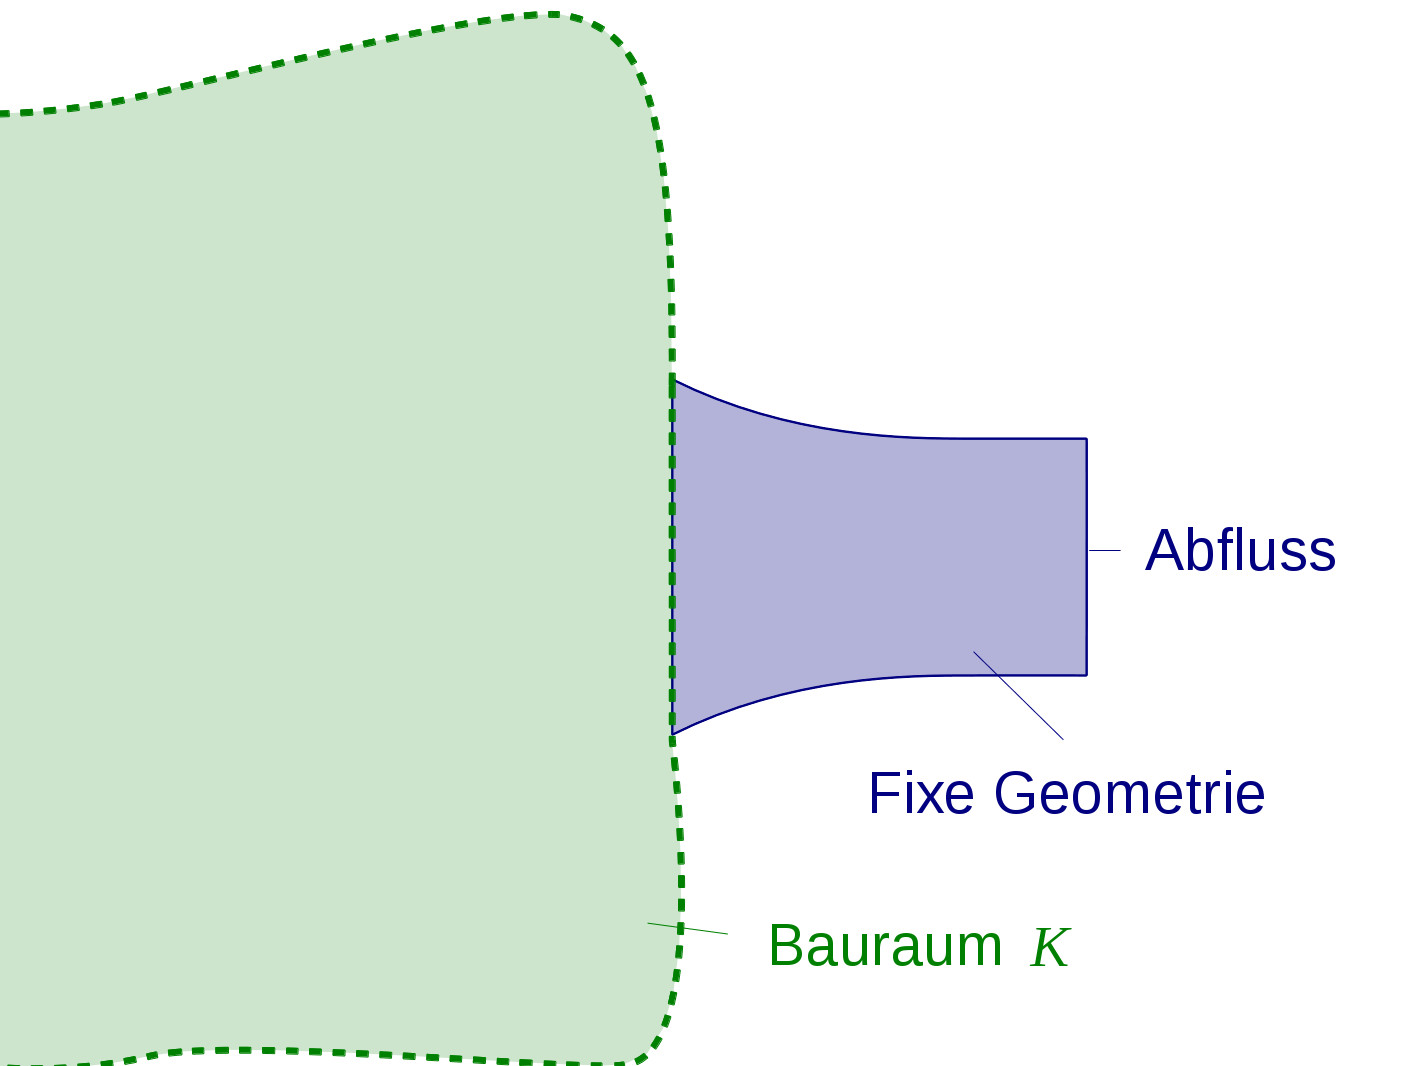
\includegraphics[scale=0.3]{skizze_DSfix3.png}  
  %   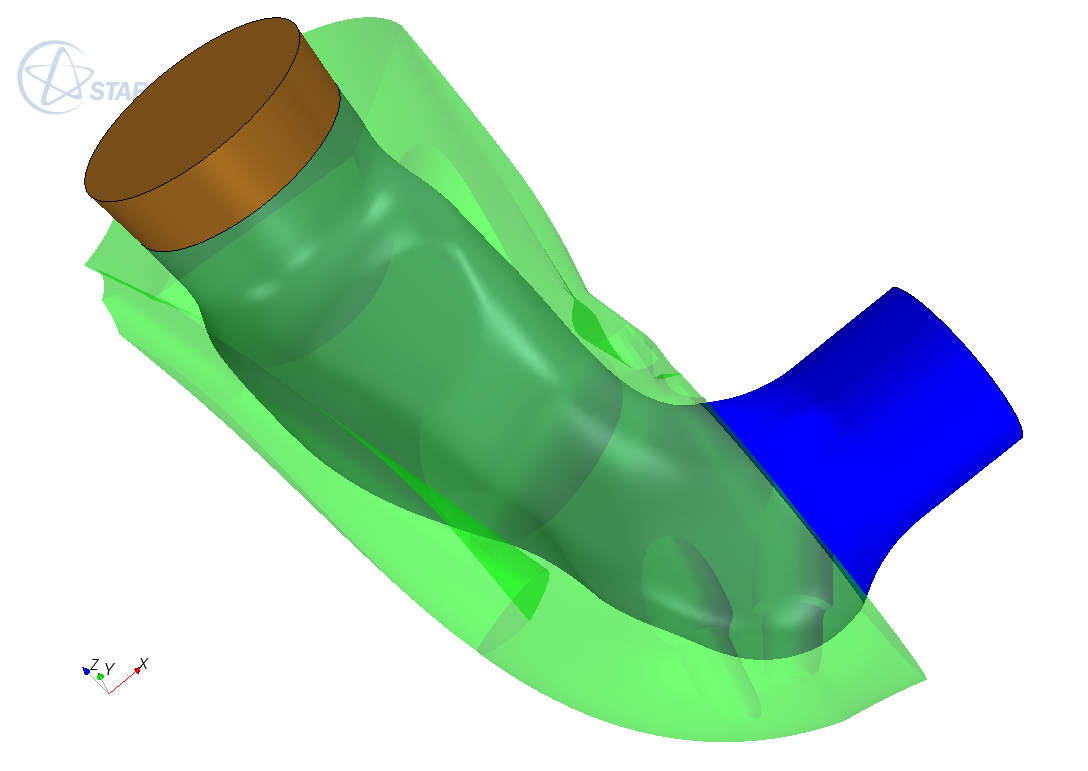
\includegraphics[scale=0.1]{darstellung_bauraum.png}  
  \end{minipage} 
  \begin{minipage}[b]{3.5 cm}
    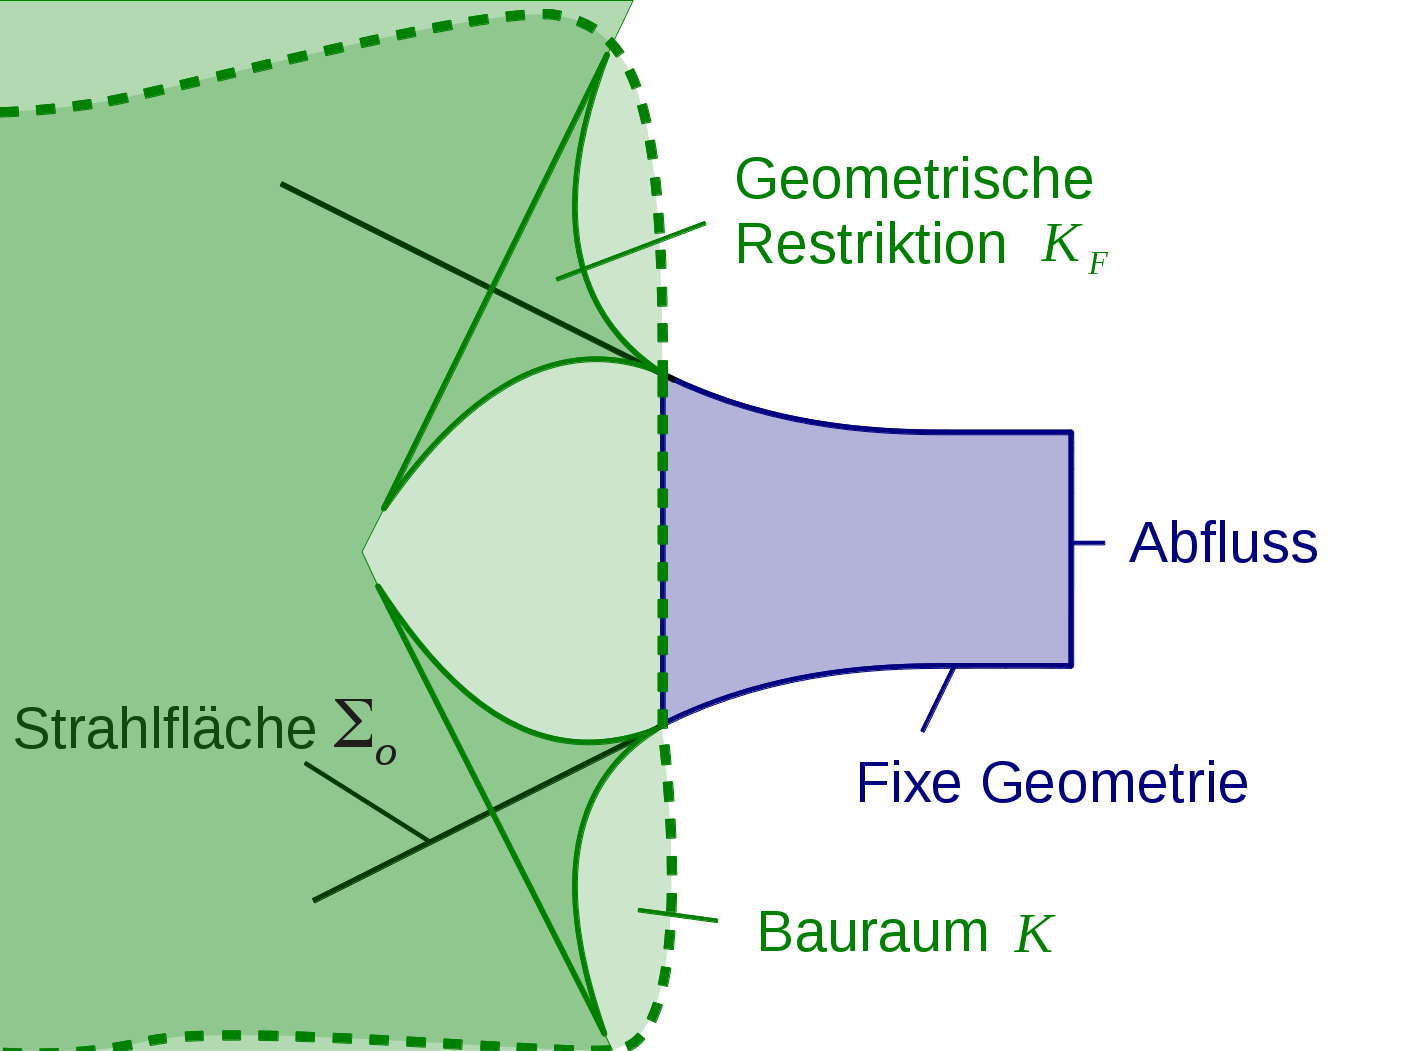
\includegraphics[scale=0.25]{skizze_DSreg.png}
  \end{minipage} 
  \begin{minipage}[b]{3 cm}
    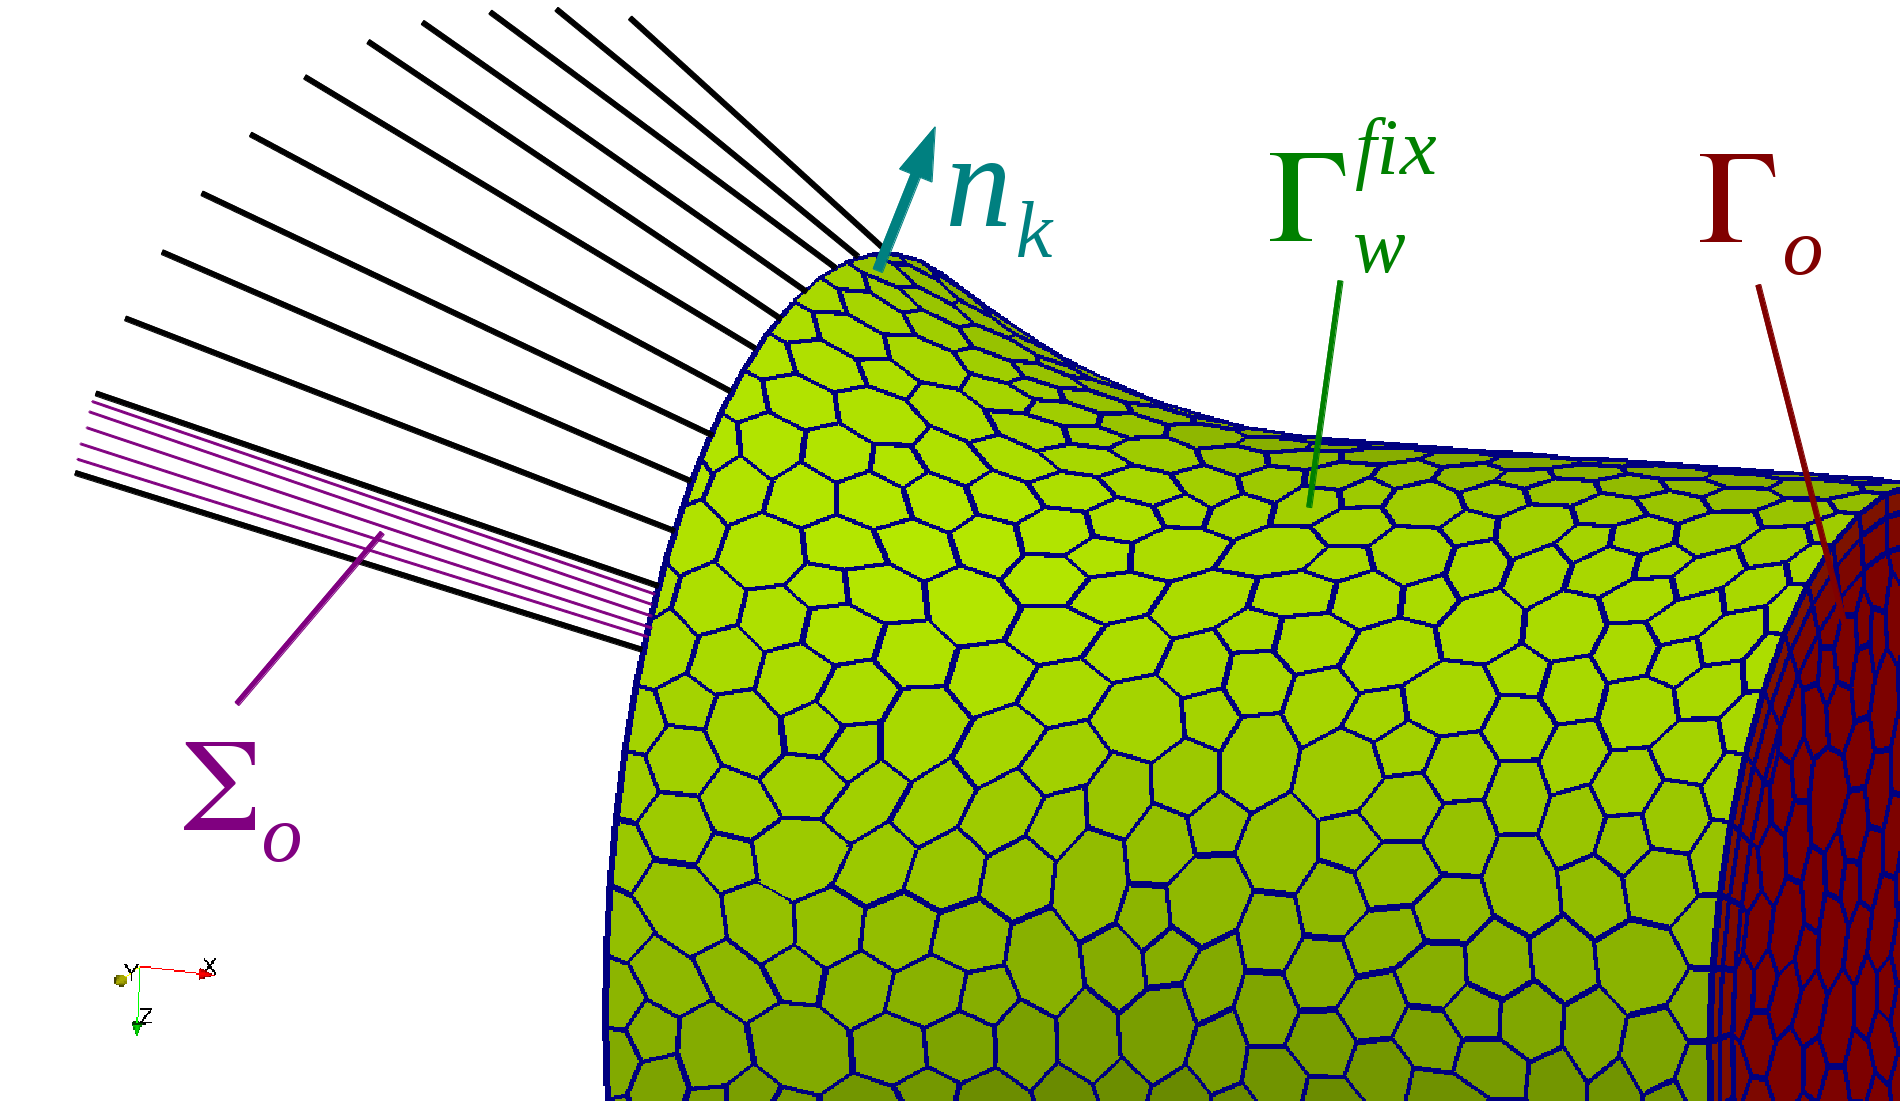
\includegraphics[scale=0.2]{strahlfl.png}  
  \end{minipage} 
  \caption{Left: fixed geometry (blue) and design space (green). 
  %\newline \textcolor{white}{.} \qquad \quad \; 
  Middle: additional valid domain.
  \newline \textcolor{white}{.} \qquad \quad \; Right: continuation of the fixed geometry.}
\label{strahlfl0}
\end{figure}
\noindent\rule{11cm}{0.4pt}
The sensitivity is calculated by
\begin{equation*}
\partial \LL_F\left(\Om,V\right)=\int_\Gamma \ell_F \left(\Om\right) \left\langle V\left(0\right),\bnn\right\rangle
\quad \mbox{with} \; \ell_F=(d(x,K_F))^2.\qquad \qquad \qquad \qquad 
\end{equation*}
}
%
%
%\section{Formoptimierung bei Strömungen ohne Filtermodell}
%\subsection{Modell- und Vernetzungseinstellungen}
%\frame{\frametitle{K-Epsilon Turbulenzmodell}
\frame{\frametitle{Turbulence modelling for high Reynolds numbers}
For applications with high Reynolds numbers (200.000) we use a K-epsilon turbulence model.
The kinematic viscosity $\nu$ in the Navier-Stokes equations is replaced by the effective viscosity, which is the sum of kinematic and turbulent viscosity:
%Im Falle des K-Epsilon Turbulenzmodells wird die durch die Fluid-Eigenschaften festgelegte kinematische Viskosität $\nu$ durch die effektive Viskosität, welche ortsabhängig ist, ersetzt. 
%Die effektive Viskosität ist die Summe der kinematischen Viskosität und der turbulenten Viskosität:\\
$$ \nu_{eff} =  \nu + \nu_t.$$
%Dies wurde in Abschnitt \ref{RANSkeModell} behandelt:
%Anstelle der Impulsgleichung im Navier-Stokes Gleichungssystem 
Instead of the convection equation
\begin{equation}
\buu_t + \nabla \cdot \left(\buu \buu^{T} \right) -\nu \Delta \buu+ \nabla p = \bzz
\end{equation}
the equation
\begin{equation}
\buu_t + \nabla \cdot \left(\buu \buu^{T} \right) - \nabla \cdot \left( \left(\nu + \textcolor{blue}{\nu_t}\right) \nabla \buu \right) + \nabla \left(p + \frac{2}{3}k \right)  = \bzz
\end{equation}
%gelöst,  wobei $\nu_t=C_\nu \frac{k^2}{\e}$. 
is solved with $\nu_t=C_\nu \frac{k^2}{\e}$.
The kinetic energy $k$ and the dissipation $\e$ are solutions of 
\begin{eqnarray} 
\partial_t k &=& - \left(\buu \cdot \nabla\right) k 
+ \nabla \cdot \left(\left(\nu+\nu_t\right)\nabla k\right) 
+ \nu_t  \left| \nabla \buu + \nabla \buu^T\right|^2 - \e \\
\partial_t \e &=& - \left(\buu \cdot \nabla\right) \e 
+ \nabla \cdot \left(\left(\nu+\frac{\nu_t}{\sigma_\e}\right)\nabla \e\right) 
+ C_1 \frac{\e}{k}\nu_t  \left| \nabla \buu + \nabla \buu^T\right|^2 
- C_2\frac{\e^2}{k} \qquad
\end{eqnarray}
with standard model constants $C_\nu=0.09$, $C_1=1.44$, $C_2=1.92$, $\sigma_\e=1.3$.\\
$ $\\
$ $\\
$ $\\
}
%
%
\frame{\frametitle{Shape gradient $\JJ_{12}^{\alpha,\varphi}$}
Shape optimization after 20 iterations:
$ $\\
$ $\\
\begin{itemize}
\item Left: negative shape gradient. \\
$ $\\
\item Middle: part of the shape gradient related to achieve uniform outflow and minimizing the total pressure loss.\\
$ $\\
\item Right: part of the shape gradient related to the geometrical constraints.
\end{itemize}
%Anhand des negativen Formgradienten erfolgt die Gitterverschiebung (rot: Geometrie wird nach außen verschoben, blau: Geometrie wird nach innen verschoben).
%Im mittleren Bild ist jener Anteil am negativen Formgradient dargestellt, welcher zum Erzielen der gleichmäßigen Ausströmung und der Reduktion des Totaldruckverlustes beiträgt.
%Jener Anteil im Formgradient, der von der Straffunktion bezüglich Bauraum- und Übergangsrestriktion stammt, ist im rechten Bild farblich dargestellt. 
%
%
$ $\\
%
\begin{figure}[htbp]
    \begin{minipage}[b]{3.4 cm}
    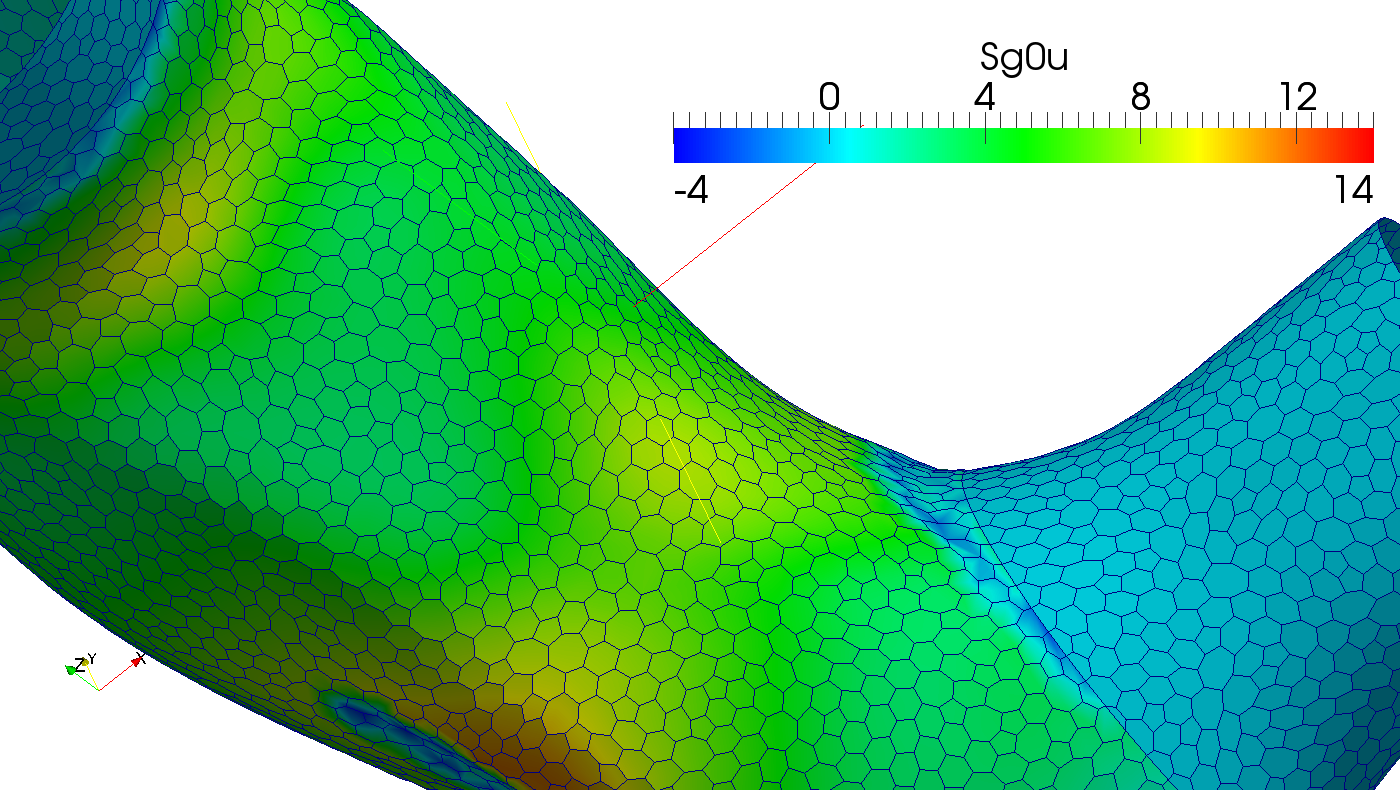
\includegraphics[scale=0.07]{RLRioJ12_Sg.png}
  \end{minipage}
    \begin{minipage}[b]{0.1 cm}
   =\\$ $\\
  \end{minipage}
  \begin{minipage}[b]{3.4 cm}
\centering
    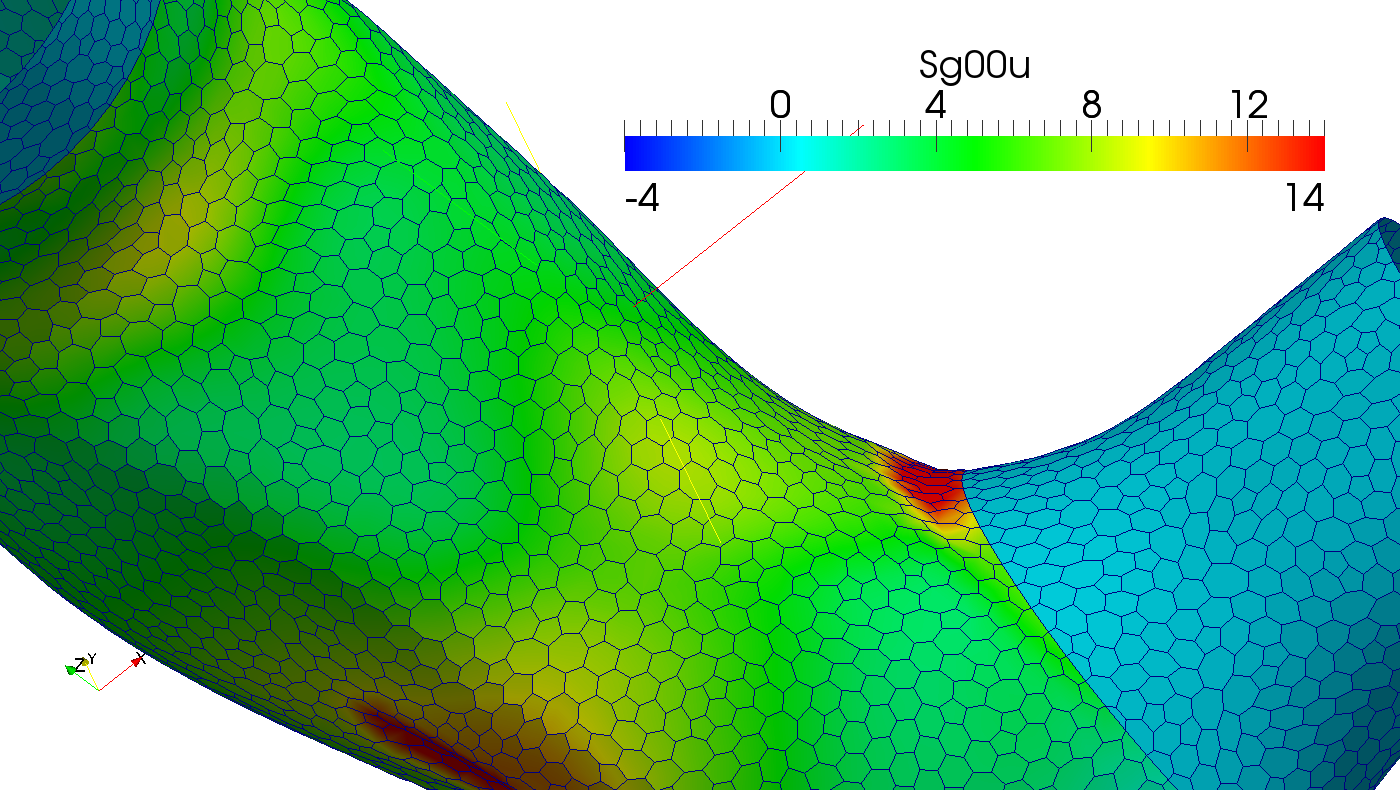
\includegraphics[scale=0.07]{RLRioJ12_Sg0.png}
  \end{minipage}
    \begin{minipage}[b]{0.1 cm}
   +\\$ $\\
  \end{minipage}
    \begin{minipage}[b]{3 cm}
    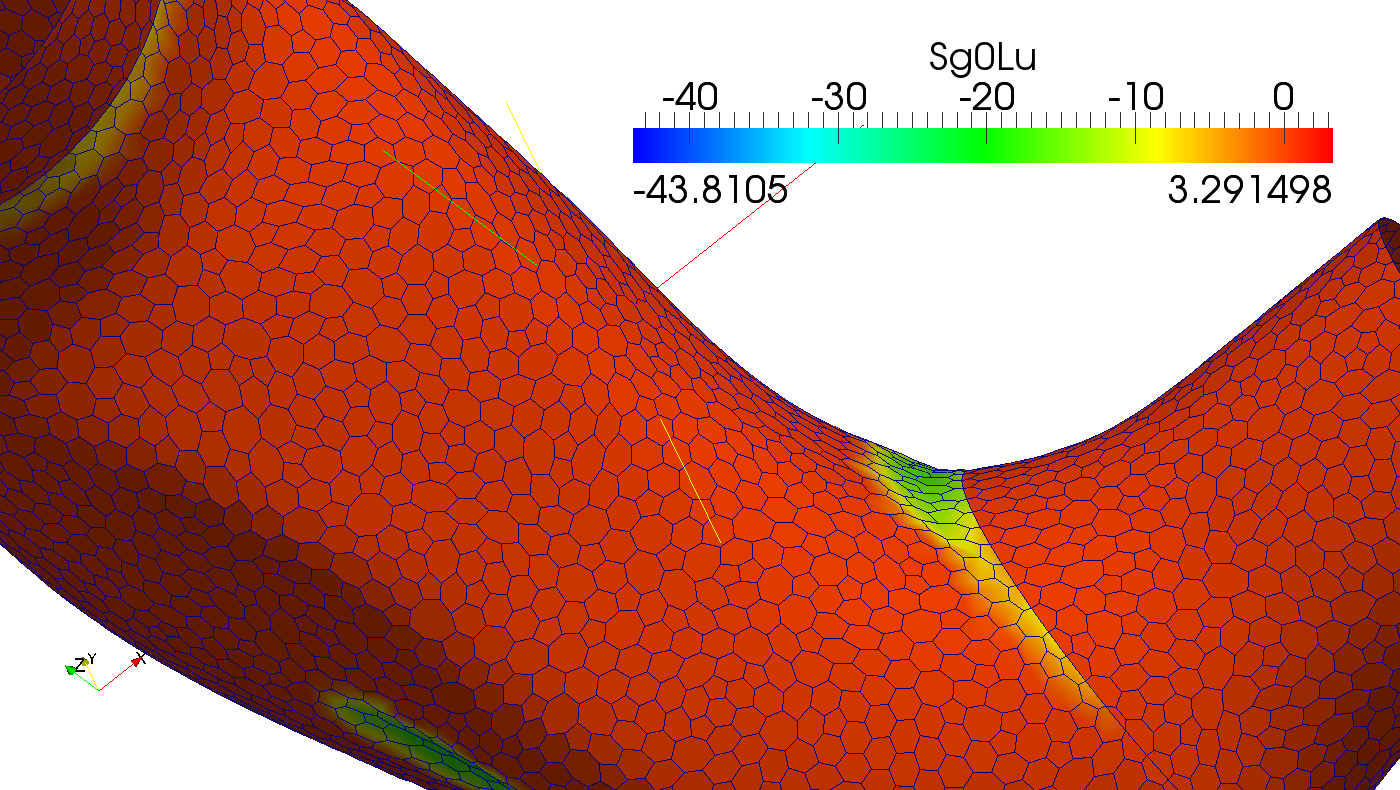
\includegraphics[scale=0.07]{RLRioJ12_SgB.png}
  \end{minipage}
 % \caption{Nach 20 Iterationen: links: negativer Formgradient; mitte: Anteile der physikalischen Zielfunktionen; rechts: Anteil durch die geometrischen Restriktionen.}
  \label{GCio4}
\end{figure}
}
\frame{\frametitle{Shape optimization with geometrical constraints for Re=200.000}
%Geometrie mit farblicher Darstellung der Änderung Ausgangsgeometrie zu den Iterationen 0, 20, 70.
Geometry with the change of geometry coloured by the distance values to the initial geometry at iteration 0, 20 70.
\begin{figure}[htbp]
    \begin{minipage}[b]{3.5 cm}
    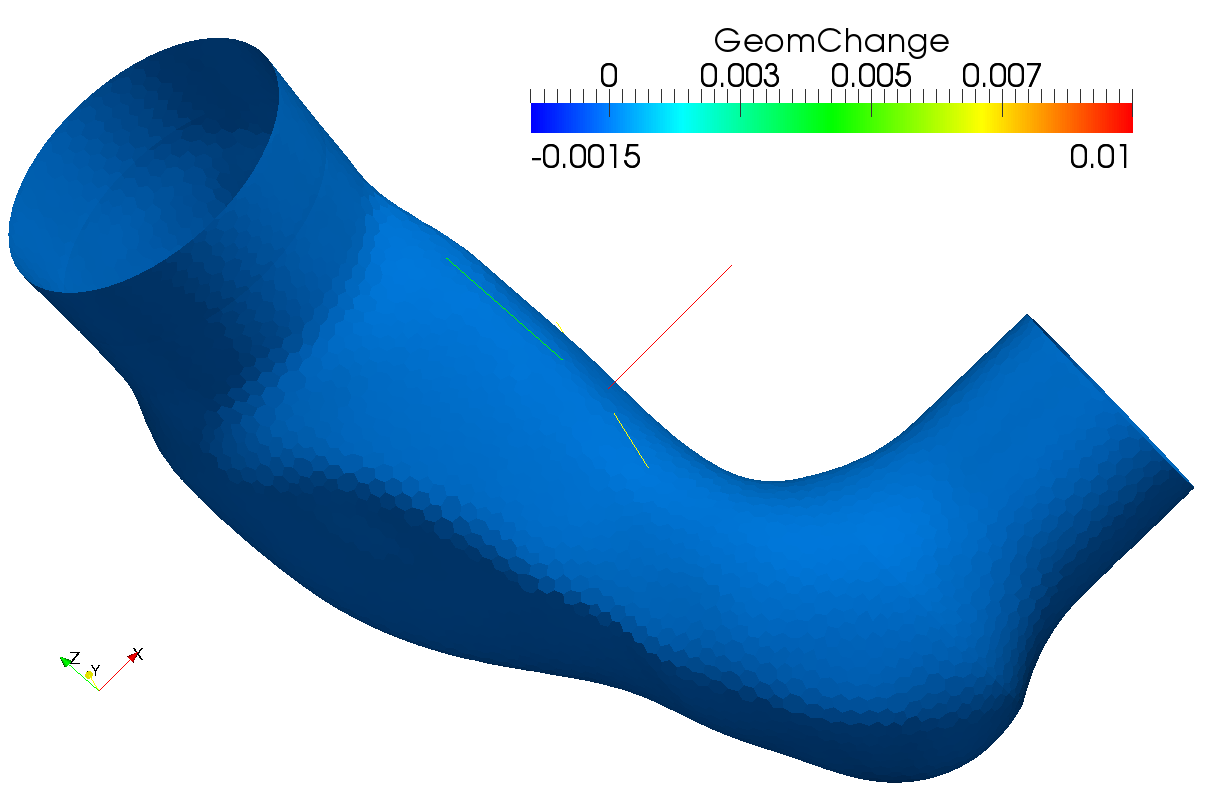
\includegraphics[scale=0.08]{RLRioJ12_v1_GC_0.png}
  \end{minipage}
  \begin{minipage}[b]{3.5 cm}
    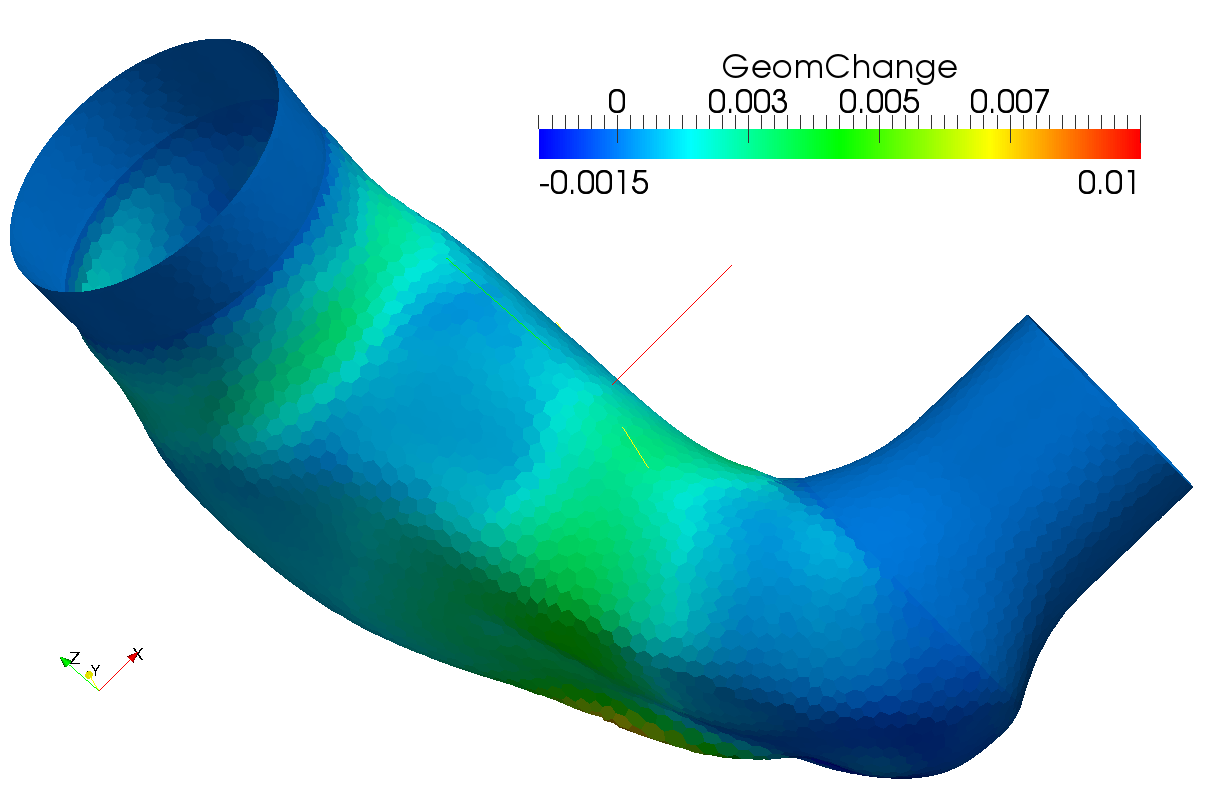
\includegraphics[scale=0.08]{RLRioJ12_v1_GC_20.png}
  \end{minipage}
    \begin{minipage}[b]{3.5 cm}
    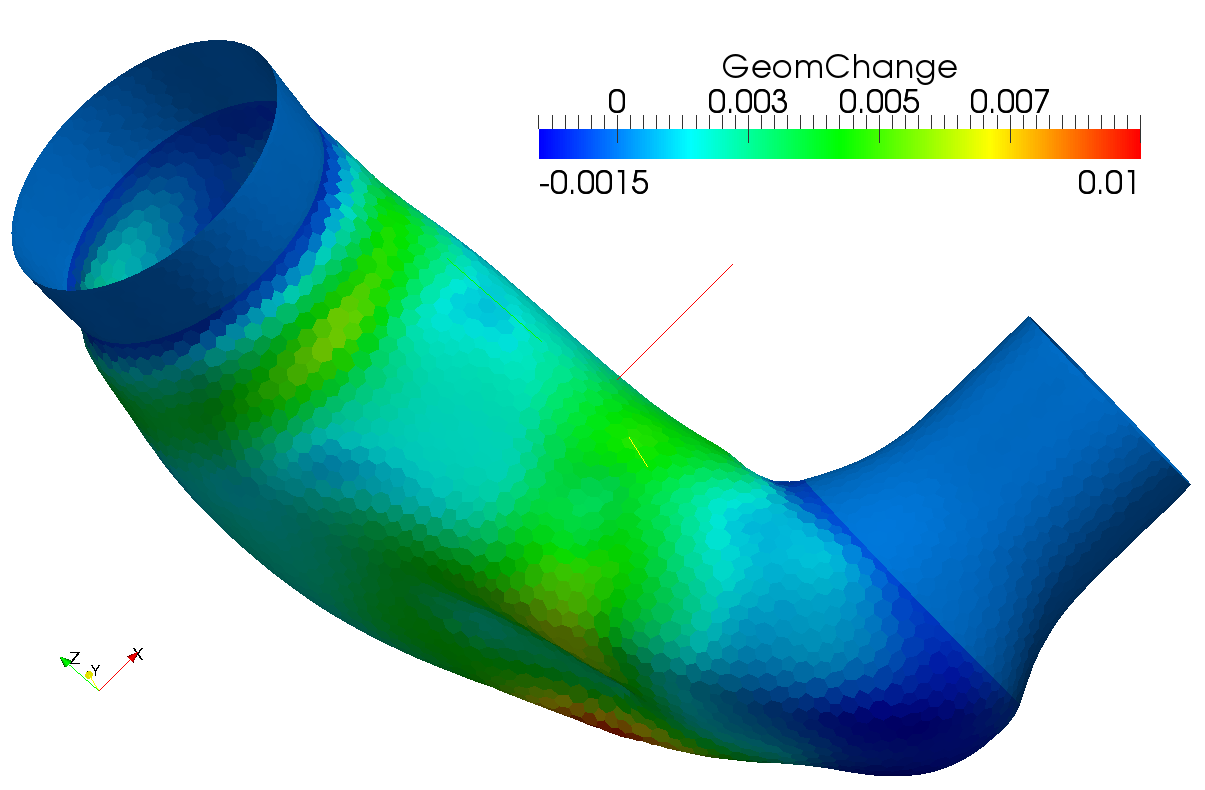
\includegraphics[scale=0.08]{RLRioJ12_v1_GC_80.png}
  \end{minipage}\\
  \begin{minipage}[b]{3.5 cm}
    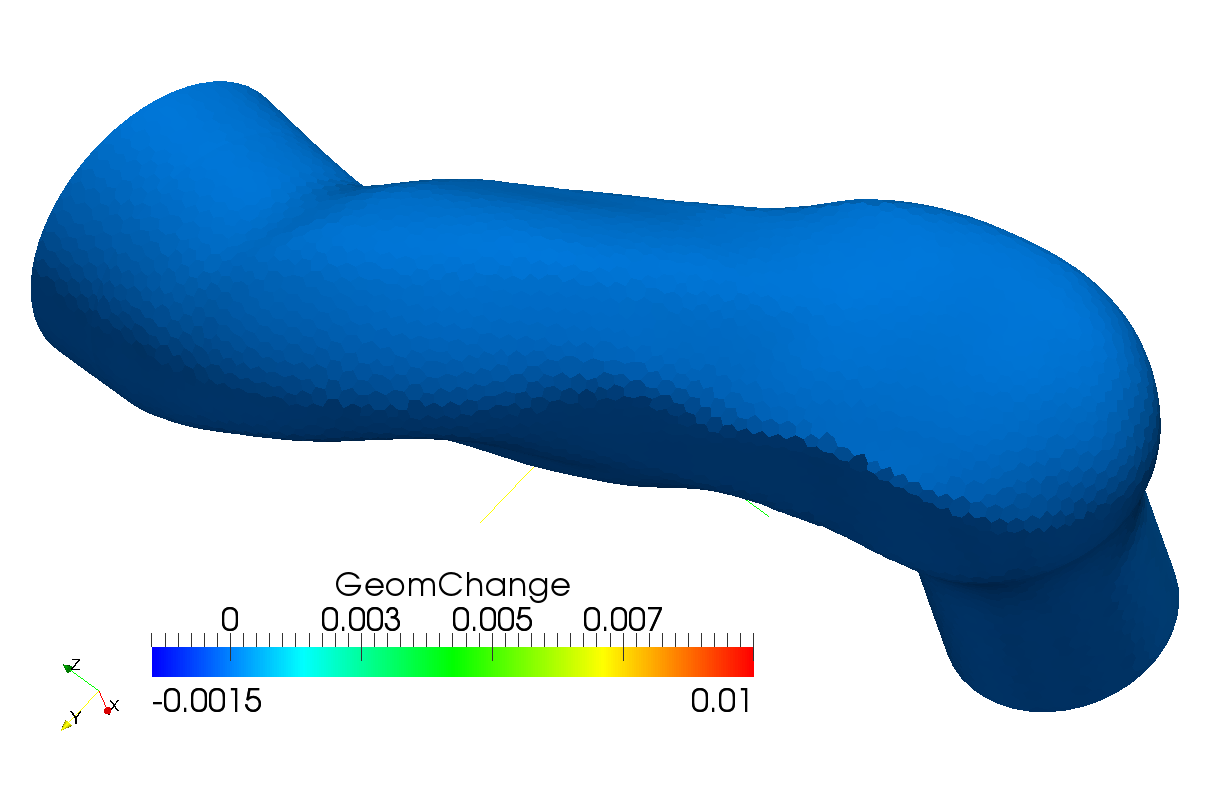
\includegraphics[scale=0.08]{RLRioJ12_v2_GC_0.png}
  \end{minipage}
    \begin{minipage}[b]{3.5 cm}
    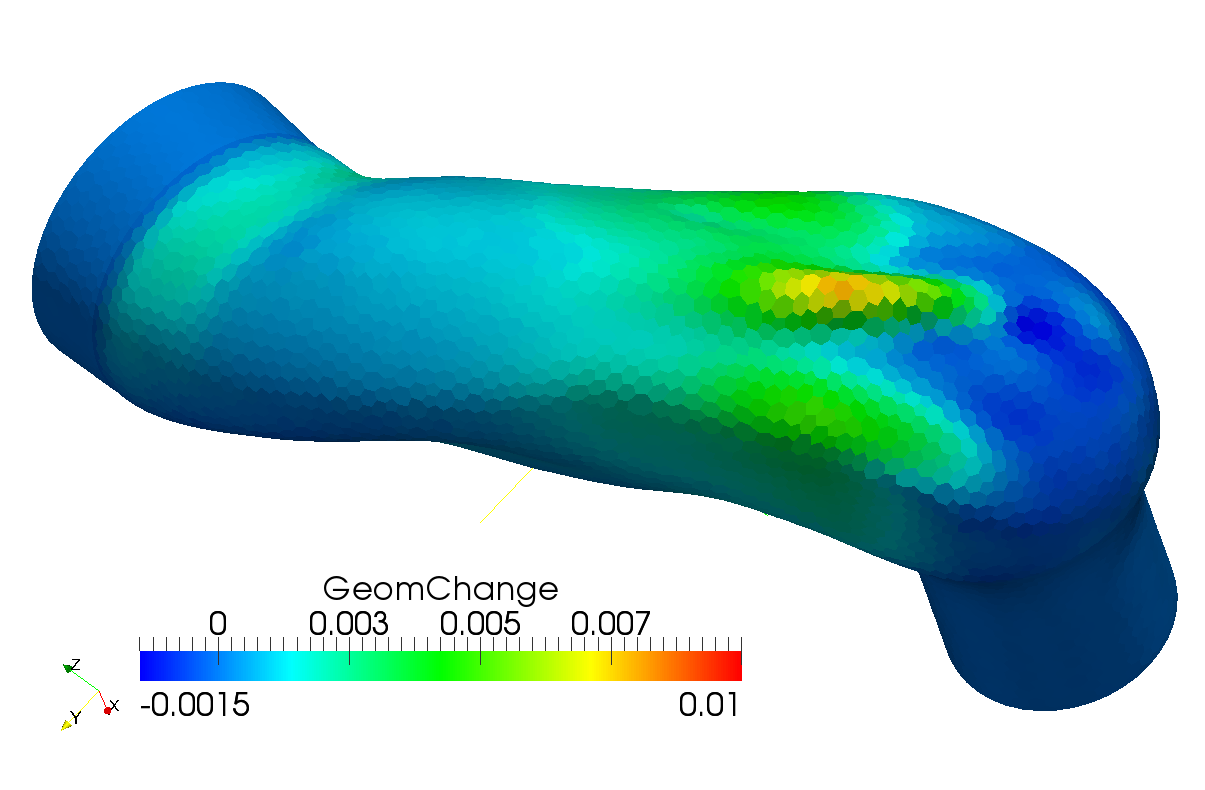
\includegraphics[scale=0.08]{RLRioJ12_v2_GC_20.png}
  \end{minipage}
  \begin{minipage}[b]{3.5 cm}
    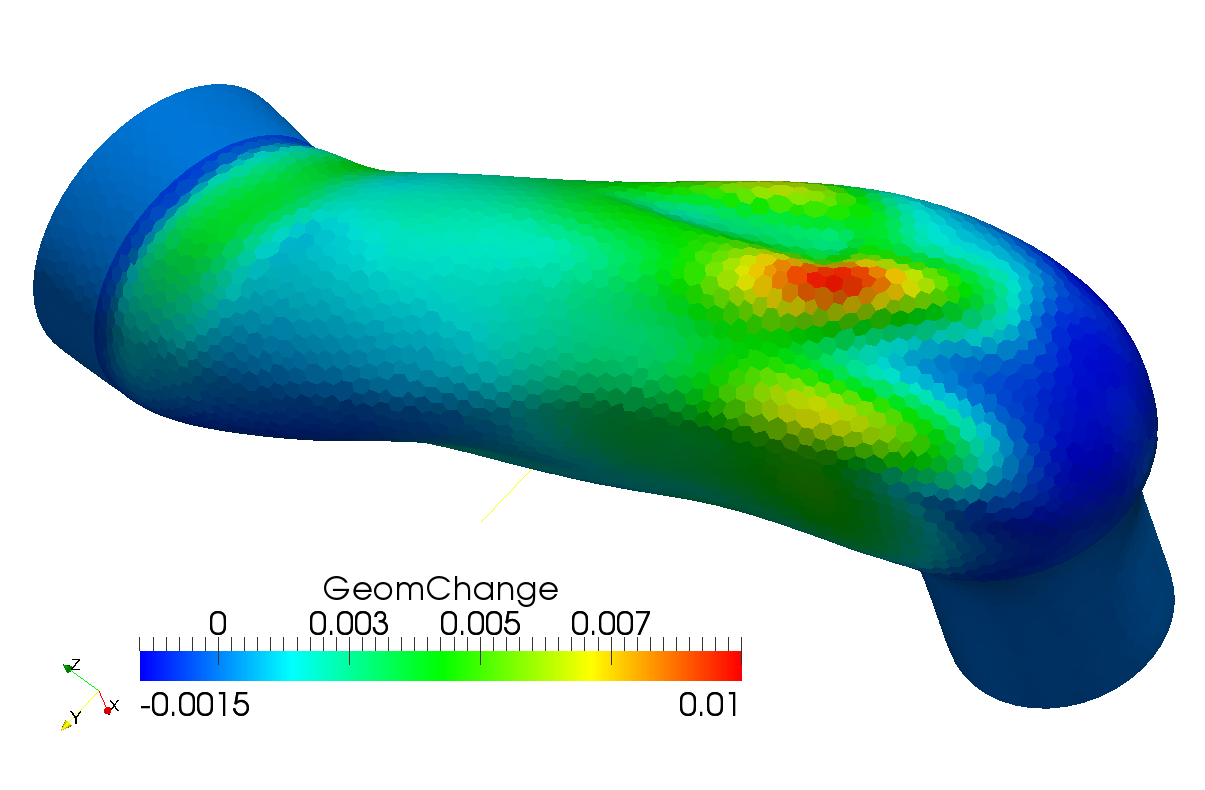
\includegraphics[scale=0.08]{RLRioJ12_v2_GC_80.png}
  \end{minipage}
%  \caption{Totaldruckverlust: Formgradient: 1.Reihe: Beginn, 2.Reihe: 20 Iterationen, 3.Reihe: 100 Iterationen.}
  \label{SGio1}
\end{figure}
}
\frame{\frametitle{Distance values to the design space}
%Die Geometrie nach 70 Iterationen und die Distanzwerte zur Bauraumgeometrie (in Meter) ist in Abbildung \ref{GCio11} dargestellt.
%Die Bauraumverletzung beträgt maximal 0.2mm. 
Geometry after 70 iterations and distance values to the design space (in meter).
The optimal geometry is at most 0.2mm outside of the design space.
\begin{figure}[htbp]
    \begin{minipage}[b]{5.5 cm}
    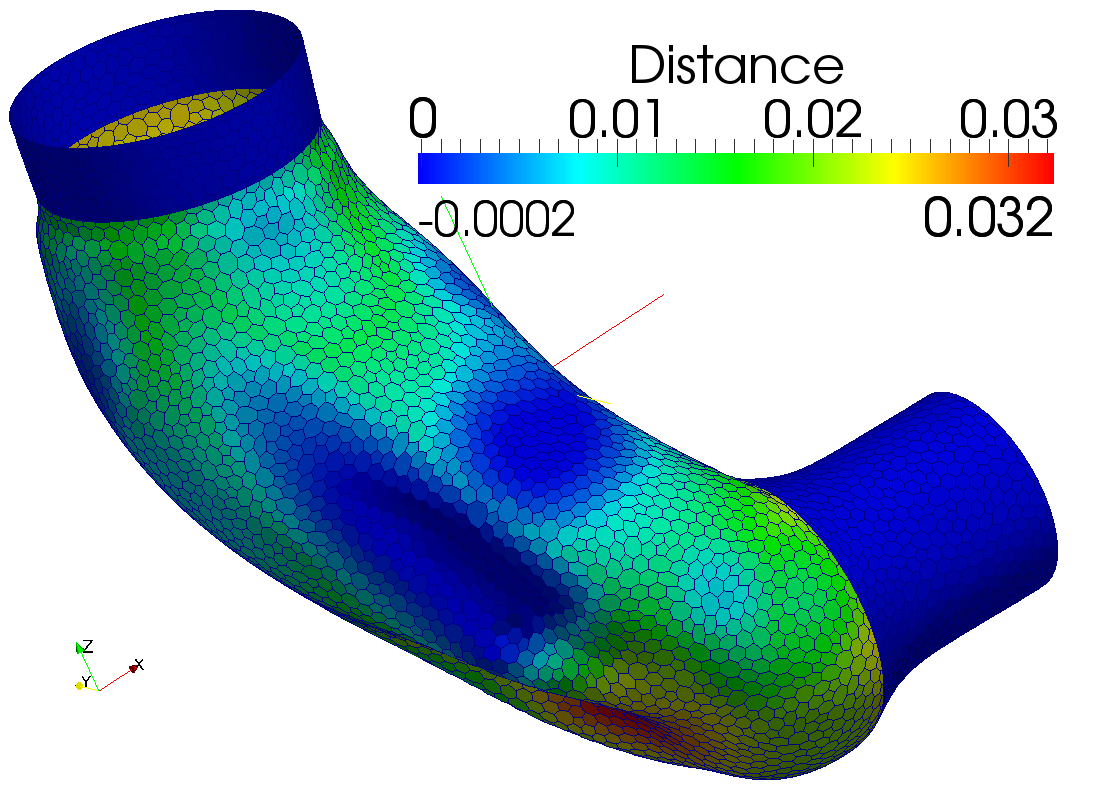
\includegraphics[scale=0.13]{RLR_J12_bauraum2.png}
  \end{minipage}
  \begin{minipage}[b]{4.5 cm}
    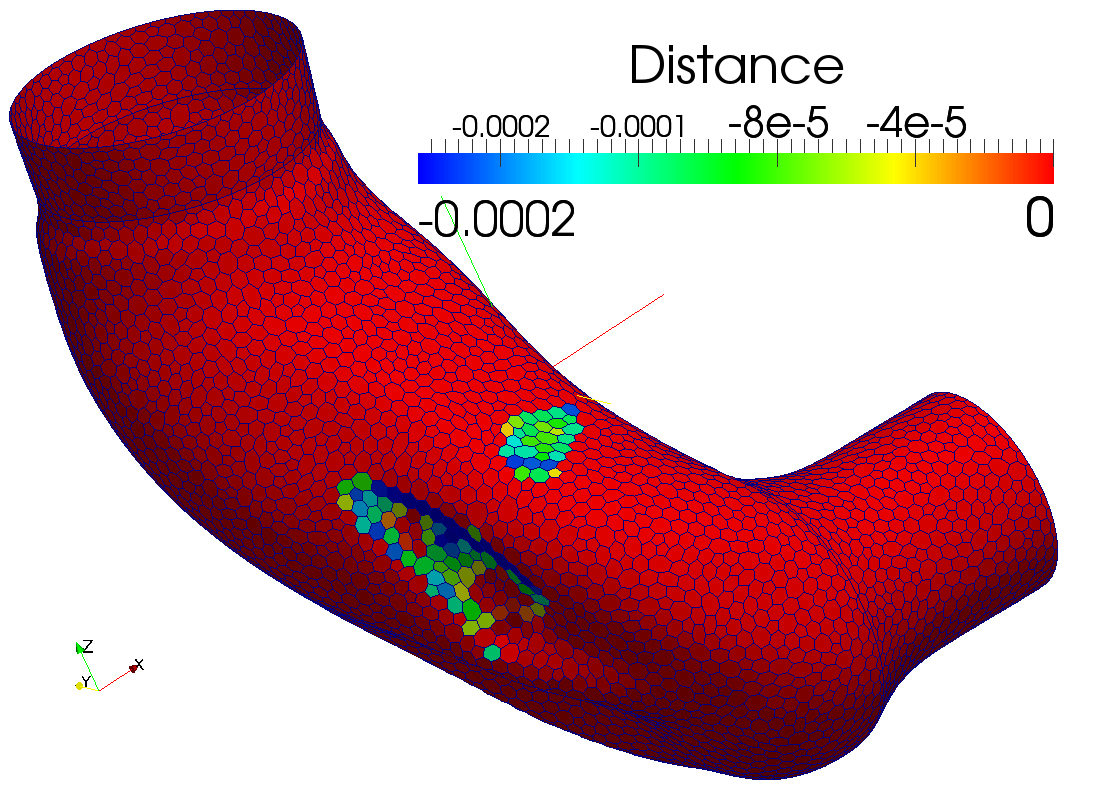
\includegraphics[scale=0.13]{RLR_J12_bauraum1.png}
  \end{minipage}
  \caption{Left: distance values. Right: distance values outside of the design space.}
  \label{GCio11}
\end{figure}
}
%
%\frame{\frametitle{Function values}
%The function values during the shape optimization are presented in the following figure:
%\begin{figure}[htbp]
%\centering
%    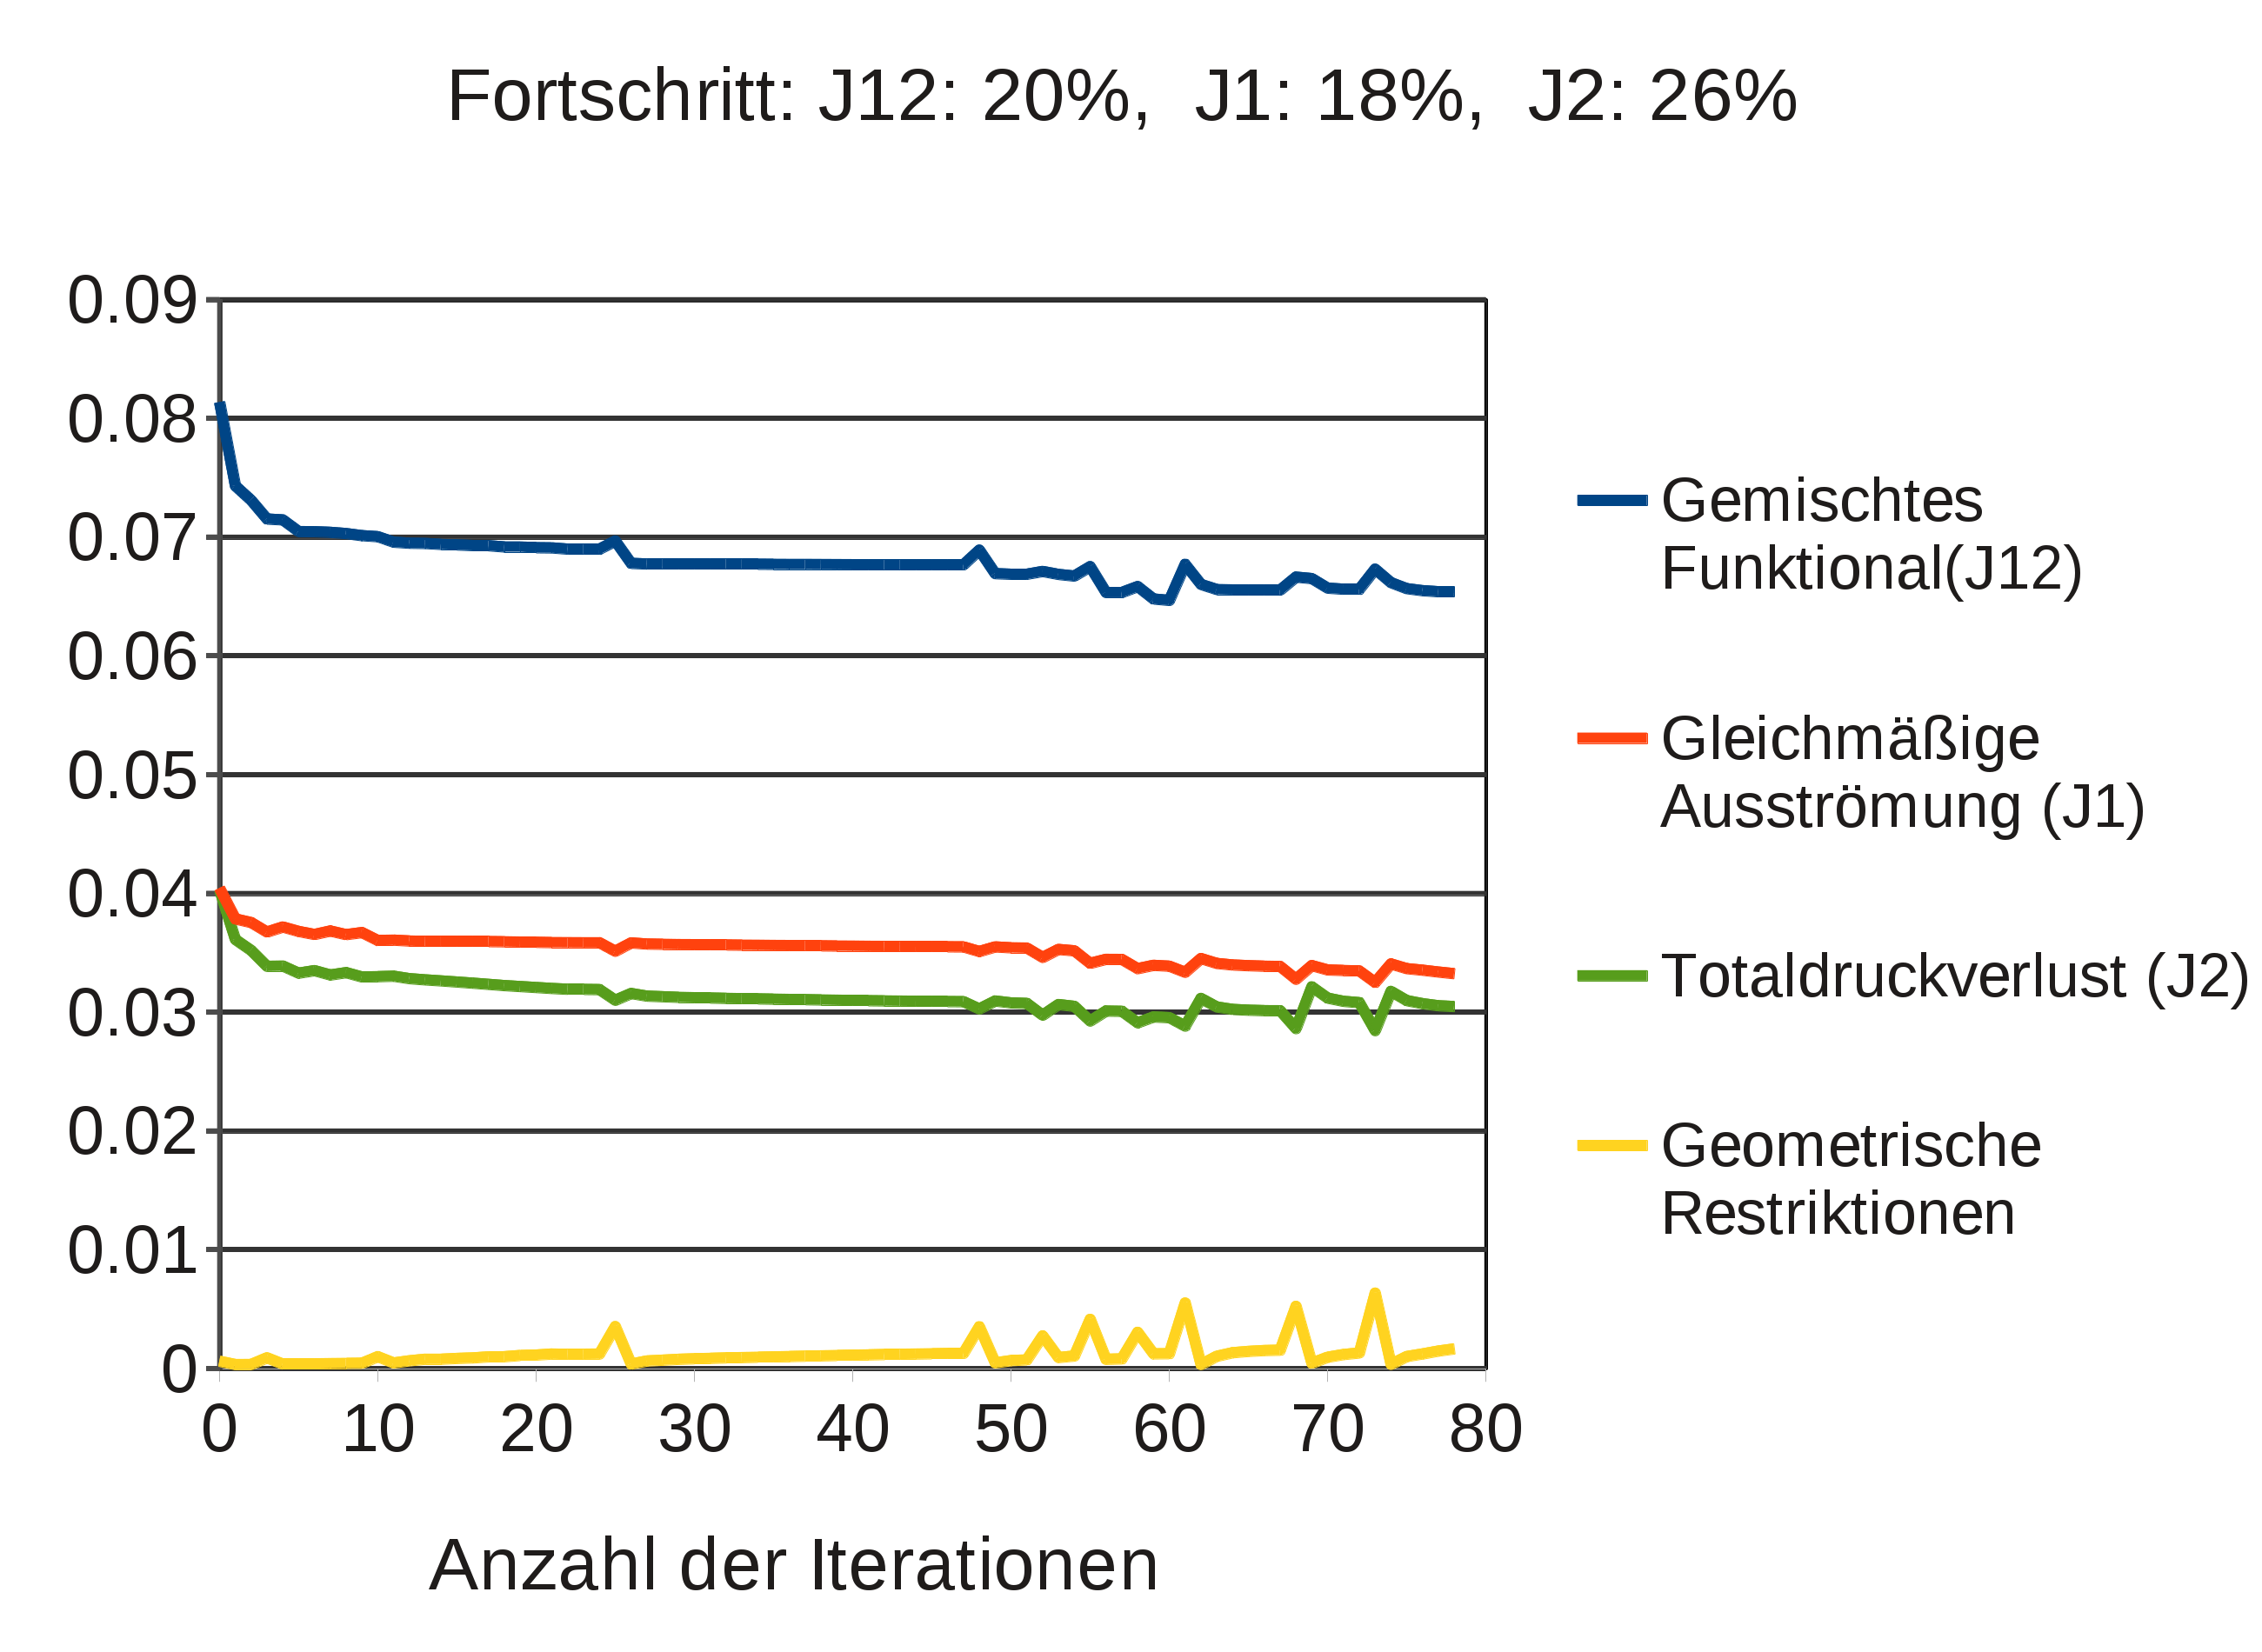
\includegraphics[scale=0.3]{RLRioJ12_fv.png}
%  %\caption{Zielfunktionswerte.}
%  \label{Skizze_funktionswerte}
%\end{figure}
%%
%}
%\frame{\frametitle{Outlet profile}
%The magnitude of the velocity on the outlet geometry at the beginning and after 60 iterations.
%%In Abbildung \ref{GCio10} ist die Geschwindigkeit an der Ausströmgeometrie zu Beginn und nach 60 Iterationen dargestellt.
%\begin{itemize}
% \item A slight progress can be visually recognized. 
%\item We emphasize to the different scaling in the figures.\\
%%Visuell ist ein leichter Fortschritt hinsichtlich gleichmäßiger Ausströmung zu erkennen. 
%%Augenmerk sollte auch auf die Skalierung der Grafiken gelegt werden. 
%%Die minimalen und maximalen Geschwindigkeiten betragen zu Beginn: 
%At the beginning: [40.22 , 72.04] and after 60 iterations: [43.31, 71.96] (m/s).
%\end{itemize}
%\begin{figure}[htbp]
%    \begin{minipage}[b]{6.6 cm}
%    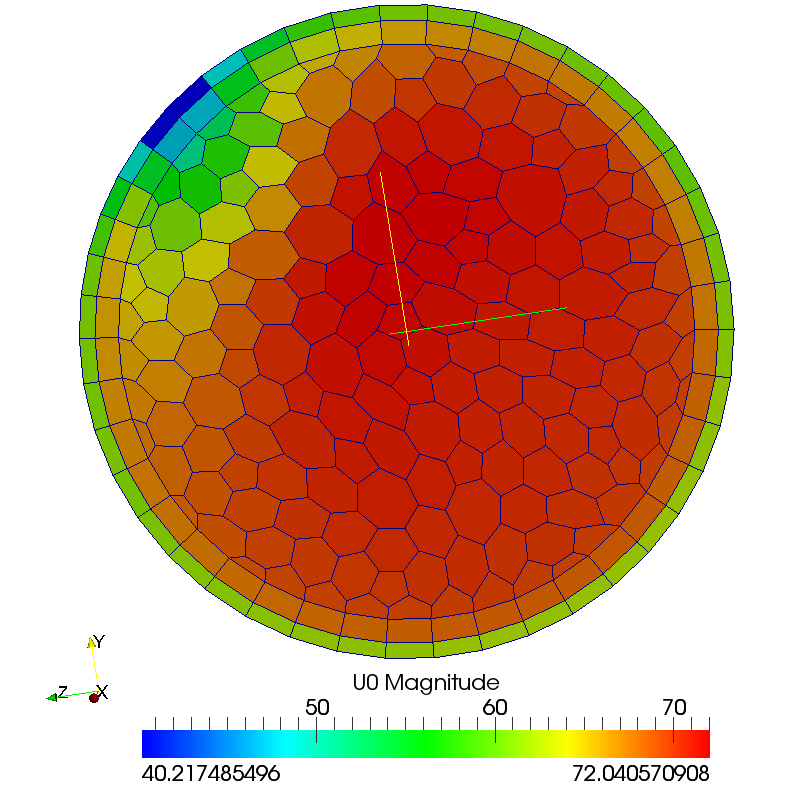
\includegraphics[scale=0.14]{outlet_U_J12_0.png}
%  \end{minipage}
%  \begin{minipage}[b]{4 cm}
%    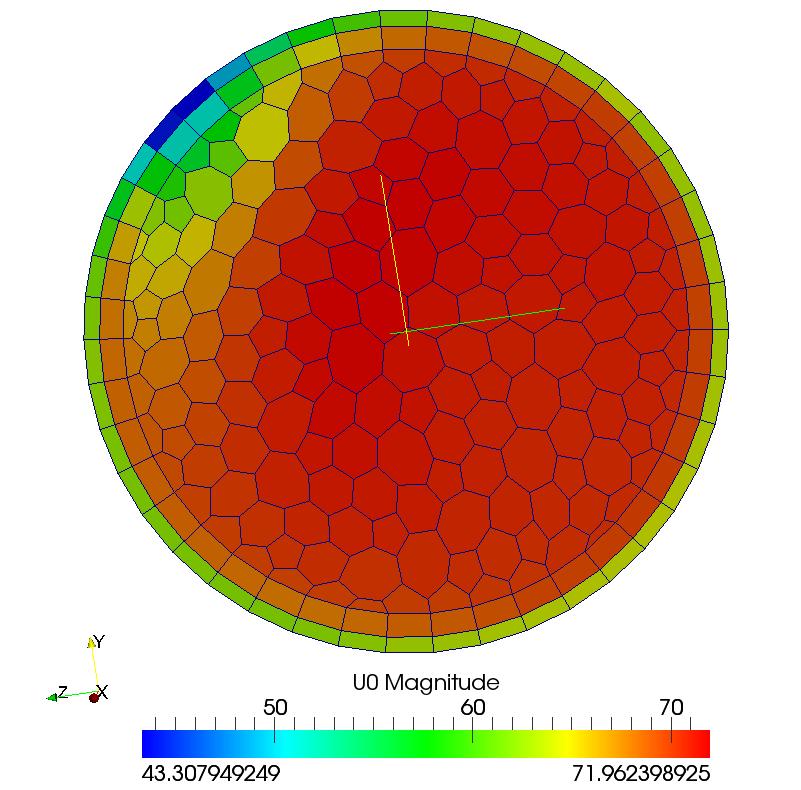
\includegraphics[scale=0.14]{outlet_U_J12_60.png}
%  \end{minipage}
%  \caption{Magnitude of the outflow-velocity: left: at the beginning, right: after 60 iterations.}
%  \label{GCio10}
%\end{figure}
%}
%\frame{\frametitle{Shape optimization tested on other geometries}
%\begin{figure}
%  \begin{minipage}[b]{6 cm}
%    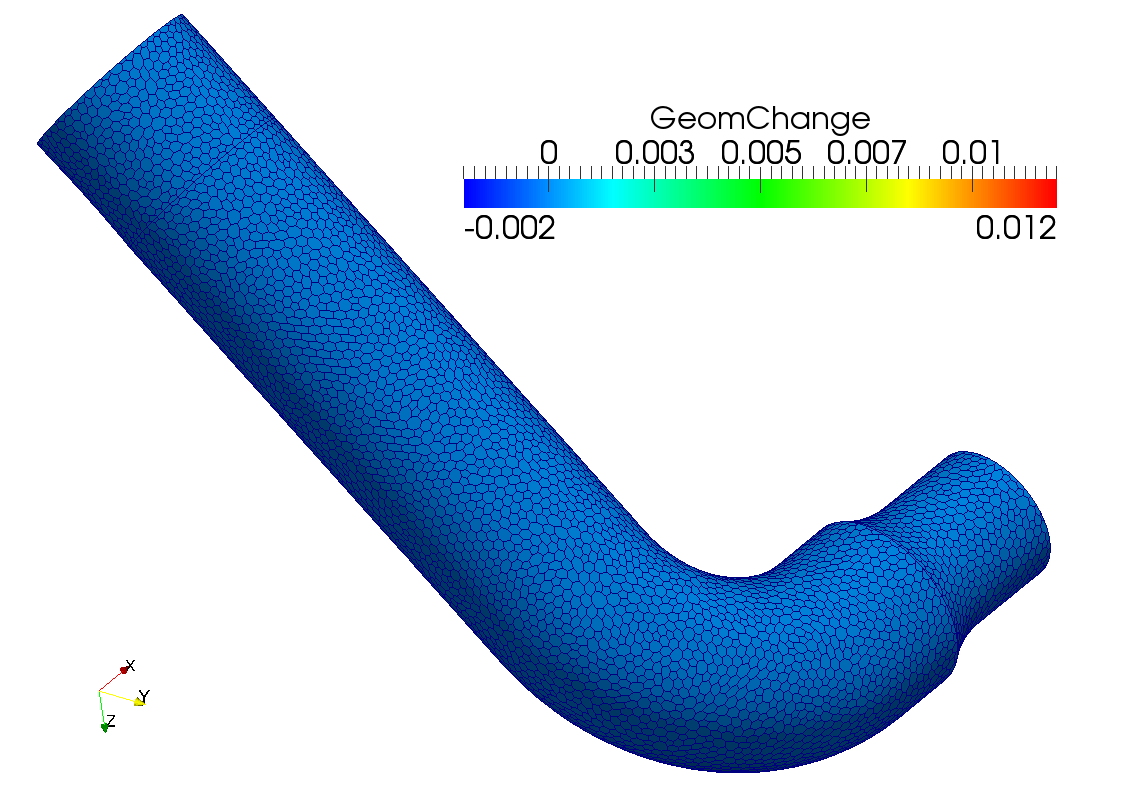
\includegraphics[scale=0.12]{Rohr1_GC0.png}
%  \end{minipage}
%  \begin{minipage}[b]{4 cm}
%    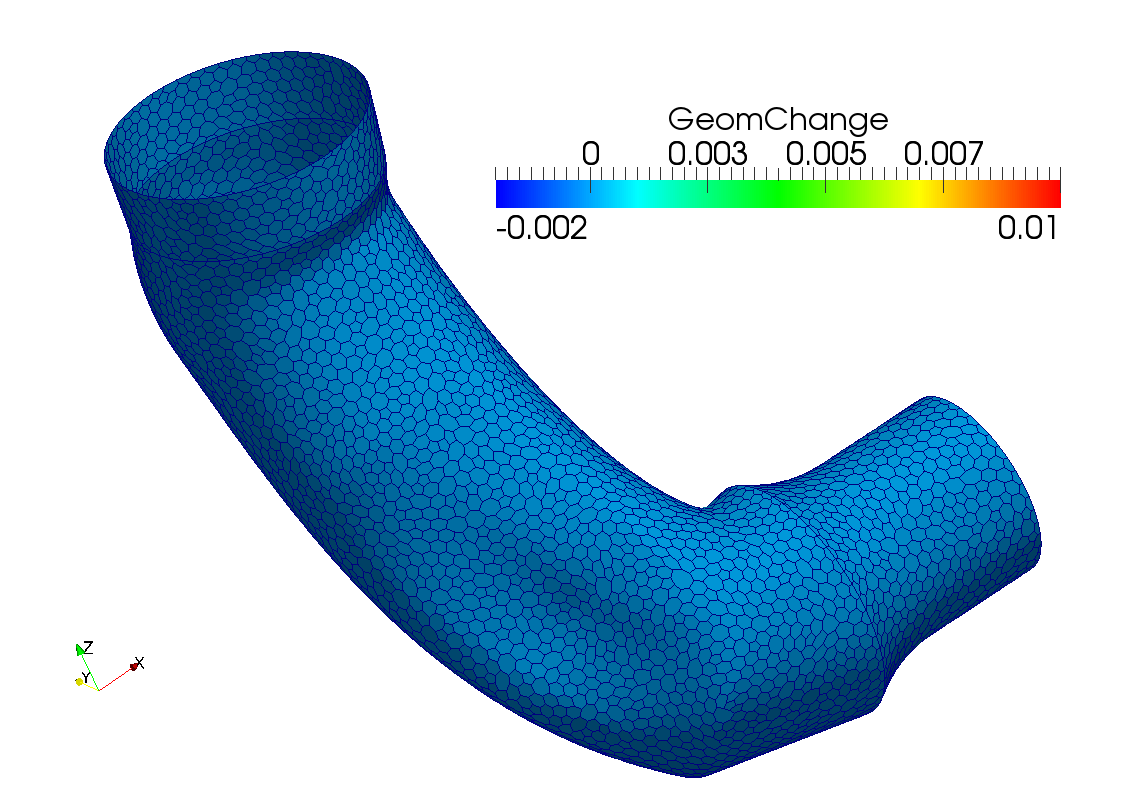
\includegraphics[scale=0.12]{RLRG1gc0.png}
%  \end{minipage}
%  \begin{minipage}[b]{6 cm}
%    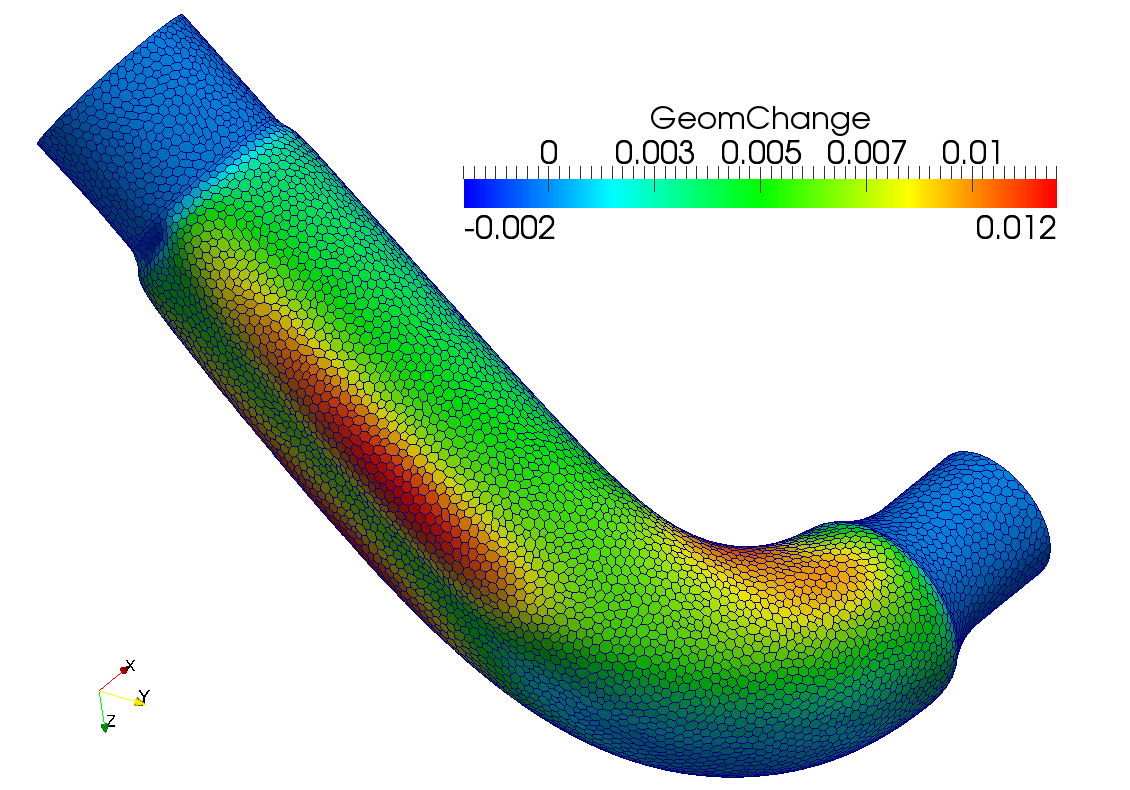
\includegraphics[scale=0.12]{Rohr1_GC80.png}
%  \end{minipage}
%  \begin{minipage}[b]{4 cm}
%    \includegraphics[scale=0.12]{RLRG1gc80.png}
%  \end{minipage}
%  \caption{Initial geometry and geometry after 80 optimization steps 
%\newline \textcolor{white}{.} \qquad \quad \; \; 
%  coloured by the change to the initial geometry.
%\newline \textcolor{white}{.} \qquad \quad \; \;
%  Left:$\JJ_1: 25\%, \JJ_2: 20 \% $,  right: $\JJ_1: 35\%, \JJ_2: 45 \% $.}
%%  \caption{Formoptimierte Geometrie mit Änderung zur Ausgangsgeometrie nach 10 Iterationen.}
%\end{figure}
%}
%\frame{\frametitle{Shape optimization tested on other geometries}
%\begin{figure}
%  \begin{minipage}[b]{5.9 cm}
%    \includegraphics[scale=0.137]{Rohr1_in0.png}
%  \end{minipage}
%  \begin{minipage}[b]{4.8 cm}
%    \includegraphics[scale=0.137]{Rohr1_out0.png}
%  \end{minipage}
%%  \begin{minipage}[b]{6 cm}
%%    \includegraphics[scale=0.12]{Rohr1_in100.png}
%%  \end{minipage}
%%  \begin{minipage}[b]{4 cm}
%%    \includegraphics[scale=0.12]{Rohr1_out100.png}
%%  \end{minipage}
%  \caption{Geometry at the beginning, coloured by  
%\newline \textcolor{white}{.} \qquad \quad \; \; 
% the change to the initial geometry and the magnitude of the velocity at the outlet.
%\newline \textcolor{white}{.} \qquad \quad \; \;
%  \textbf{Left}: inlet, \textbf{right}: outlet. 
%\newline \textcolor{white}{.} \qquad \quad \; \;
%$\JJ_1: 25\%, \JJ_2: 20 \% $.}
%%  \caption{Formoptimierte Geometrie mit Änderung zur Ausgangsgeometrie nach 10 Iterationen.}
%\end{figure}
%}
%\frame{\frametitle{Shape optimization tested on other geometries}
%\begin{figure}
%%  \begin{minipage}[b]{6 cm}
%%    \includegraphics[scale=0.12]{Rohr1_in0.png}
%%  \end{minipage}
%%  \begin{minipage}[b]{4 cm}
%%    \includegraphics[scale=0.12]{Rohr1_out0.png}
%%  \end{minipage}
%  \begin{minipage}[b]{5.9 cm}
%    \includegraphics[scale=0.137]{Rohr1_in100.png}
%  \end{minipage}
%  \begin{minipage}[b]{4.8 cm}
%    \includegraphics[scale=0.137]{Rohr1_out100.png}
%  \end{minipage}
%  \caption{Geometry after 80 optimization steps, coloured by  
%\newline \textcolor{white}{.} \qquad \quad \; \; 
% the change to the initial geometry and the magnitude of the velocity at the outlet.
%\newline \textcolor{white}{.} \qquad \quad \; \;
%  \textbf{Left}: inlet, \textbf{right}: outlet. 
%\newline \textcolor{white}{.} \qquad \quad \; \;
%$\JJ_1: 25\%, \JJ_2: 20 \% $.}
%%  \caption{Formoptimierte Geometrie mit Änderung zur Ausgangsgeometrie nach 10 Iterationen.}
%\end{figure}
%}

%% \frame{\frametitle{Aspects on the mesh: checkGeometry, boundary layer structure}
%% The used OpenFOAM routine \textcolor{dblue}{checkGeometry} \begin{footnotesize} (\$FOAM\_APP/utilities/mesh/manipulation/checkMesh ) \end{footnotesize} ensures some 
%% \begin{columns}[c]
%% \column[c]{3.8cm}
%% \begin{itemize}
%% \item general mesh properties:
%% \begin{itemize}
%% \item closedCells, 
%% \item zeroVolumeCells,
%% \item zeroAreaFace, ...
%% \end{itemize}
%% \end{itemize}
%% \column{0.6cm}and 
%% $ $\\
%% $ $\\
%% $ $\\
%% \column{3.9cm}
%% \begin{itemize}
%% \item mesh quality properties:
%% \begin{itemize}
%% \item faceSkewness (figure), 
%% \item flatnessFace,
%% \item highAspectRatioCells, ...
%% \end{itemize} 
%% \end{itemize}
%% \column{2cm}
%% \includegraphics[scale=0.3]{skewnessAngle.png}
%% \end{columns}
%% \noindent\rule{10cm}{0.4pt}\\
%% To ensure \textcolor{dblue}{boundary layer structure} between fixed geometry and optimizing geometry the splitting of geometries by planar interfaces should be avoided.
%% \begin{figure}[htbp]
%%   \centering
%%    \includegraphics[scale=0.37]{VernetzungAzoom.png}
%%      \includegraphics[scale=0.065]{RLRhighReInterface23.png}
%%    \includegraphics[scale=0.065]{RLRhighReInterface23large.png}\\
%%    \includegraphics[scale=0.37]{VernetzungBzoom.png}
%%      \includegraphics[scale=0.065]{RLR2e5noInterface.png}
%%    \includegraphics[scale=0.065]{RLR2e5noInterfaceLong.png}
%% \caption{Upper: involving planar interfaces, \qquad \qquad
%% \newline \textcolor{white}{.} \qquad  \qquad \,
%% lower: without interfaces to preserve layer structure.}
%% \end{figure}
%% }
%% \frame{\frametitle{Aspects on the mesh: Avoiding volume loss}
%% \begin{figure}
%% \begin{minipage}[b]{5.6 cm}
%% \textbf{Volume loss}:\\
%% In case the mesh quality creteria are not satisfied a remeshing is necessary.
%% The way of meshing from a stl surface in Star-CD CCM+ leads to dislocations of the geometry (depending on the curvature). 
%% \end{minipage}
%% \begin{minipage}[b]{5 cm}
%%   \centering
%%     \includegraphics[scale=0.05]{stl_0_1_10.png} \qquad 
%%     \includegraphics[scale=0.05]{stl_0_1_10_zoom.png}
%%  % \caption{Links: bisherige Variante. Rechts: Variante zur Vermeidung des Volumenverlustes.}
%% \end{minipage}
%% \end{figure}
%% $ $\\
%% \textbf{Avoiding dislocations at the in-/outlet:}
%% \begin{itemize}
%% \item fixed surface at the in-/outlet will be kept
%% \item optimizing surface will be renewed during remeshing
%% \item stitch surface data at the interface to preserve a connected surface mesh 
%% \end{itemize}
%% \begin{figure}[htbp]
%%   \centering
%%     \includegraphics[scale=0.4]{flex_geom2c.png} 
%%     \includegraphics[scale=0.4]{flex_geom3c.png}
%%     \includegraphics[scale=0.1]{fix_volRed.png}
%% %  \caption{\textbf{Links}: bisherige Variante.
%% %\newline \textcolor{white}{.} \qquad \qquad \qquad  
%% % \textbf{Rechts}: Variante zur Vermeidung des Volumenverlustes.}
%% \end{figure}
%% $ $\\
%% $ $\\
%% }

\frame{\frametitle{Laplace-Beltrami smoothing}
\textcolor{dblue}{Equation on the surface $\Gamma$:}
\begin{eqnarray}
 -\varepsilon \Delta_\Gamma w + w &=& -g_{\JJ_{12}}  \qquad \mbox{auf}\quad \Gamma,\\
w &=& 0 \qquad \qquad \, \mbox{auf}\quad \partial \Gamma.
\end{eqnarray}
$ $\\
\textcolor{dblue}{Benefits of the Laplace-Beltrami usage:}
\begin{itemize}
\item Higher regularity of each grid movement.
\item Keeping the property of a descent direction.
\item Preconditioning gradient method.
\end{itemize}
$ $\\
\textcolor{dblue}{Notes on the numerical realiszation:} 
\begin{itemize}
\item Usage of a triangulated surface mesh - grid management in OpenFOAM.
\item Discretization with finite elemets 3D tent function.
\item Efficient storage of sparse matrix and usage of iterative solver.
\end{itemize}
\begin{figure}[htbp]
\begin{minipage}[b]{4 cm}
Linear \textcolor{dred}{basis functions $\varphi_j$} on a triangulated surface with common support \textcolor{dgreen}{$supp\left(\varphi_1 \varphi_2\right) \neq 0$}.\\
$ $\\
  \end{minipage}
\begin{minipage}[b]{5 cm}
    \includegraphics[scale=0.6]{femHut1.png} 
  \end{minipage}
\end{figure}
$ $\\
$ $\\
}

\frame{\frametitle{Laplace-Beltrami smoothing: numerical results}
\begin{figure}[htbp]
  \centering
    \includegraphics[scale=0.1]{Rohr3_lb0.png} 
    \includegraphics[scale=0.1]{Rohr3_lb1.png} \qquad
    \\
    \includegraphics[scale=0.1]{TOR_LB0.png} 
    \includegraphics[scale=0.1]{TOR_LB1.png}  
    \\
    \begin{minipage}[b]{3.9 cm}
\begin{footnotesize}
\begin{eqnarray*}
 -\varepsilon \Delta_\Gamma w + w &=&  -g_{\JJ_{12}}  \;\; \mbox{auf}\, \Gamma,\\
w &=& 0 \qquad \quad \,\; \mbox{auf}\, \partial \Gamma.
\end{eqnarray*} 
\end{footnotesize}
\end{minipage}
  \caption{Left: without LB-smoothing, middle: using LB-smoothing.}
\end{figure}
%$ $\\
%\begin{eqnarray}
% -\varepsilon \Delta_\Gamma w + w &=& -g_{\JJ_{12}}  \qquad \mbox{auf}\quad \Gamma\\
%w &=& 0 \qquad \qquad \, \mbox{auf}\quad \partial \Gamma
%\end{eqnarray}
%$ $\\
}
%
%
%
%\frame{\frametitle{Shape optimization on different geometries and Re-numbers}
%\begin{figure}
%  \begin{minipage}[b]{6 cm}
%    \includegraphics[scale=0.12]{B120R200I0.png}
%  \end{minipage}
%  \begin{minipage}[b]{4 cm}
%    \includegraphics[scale=0.12]{M23R400o1i0.png}
%  \end{minipage}
%  \begin{minipage}[b]{6 cm}
%    \includegraphics[scale=0.12]{T090R1000I0.png}
%  \end{minipage}
%  \begin{minipage}[b]{4 cm}
%    \includegraphics[scale=0.12]{I120R2e5I0.png}
%  \end{minipage}
%  \caption{Initial geometries: upper: Re = 200, \; Re = 400; \qquad \qquad
%\newline \textcolor{white}{.} \qquad \qquad \qquad \qquad \qquad \qquad \,  lower: Re = 1000, Re = 200 000.}
%%  \caption{Formoptimierte Geometrie mit Änderung zur Ausgangsgeometrie nach 10 Iterationen.}
%%\includegraphics[scale=0.13]{T090R1000I0.png}
%%    \includegraphics[scale=0.13]{T090R1000I30.png}
%\end{figure}
%}
\frame{\frametitle{Shape optimization tested on other geometries}
\begin{figure}
  \begin{minipage}[b]{6 cm}
    \includegraphics[scale=0.12]{B120R200I30.png}
  \end{minipage}
  \begin{minipage}[b]{4 cm}
    \includegraphics[scale=0.12]{M23R400o1i200.png}
  \end{minipage}
  \begin{minipage}[b]{6 cm}
    \includegraphics[scale=0.12]{T090R1000I30.png}
  \end{minipage}
  \begin{minipage}[b]{4 cm}
    \includegraphics[scale=0.12]{I120R2e5I15.png}
  \end{minipage}
  \caption{Final geometries: upper: Re = 200, \; Re = 400; \qquad \qquad
\newline \textcolor{white}{.} \qquad \qquad \qquad \qquad \qquad \qquad \,  lower: Re = 1000, Re = 200 000.}
%  \caption{Initial geometry and geometry after 80 optimization steps 
%\newline \textcolor{white}{.} \qquad \quad \; \; 
%  coloured by the change to the initial geometry.}
%\newline \textcolor{white}{.} \qquad \quad \; \;}
%  Left:$\JJ_1: 25\%, \JJ_2: 20 \% $,  right: $\JJ_1: 35\%, \JJ_2: 45 \% $.}
%  \caption{Formoptimierte Geometrie mit Änderung zur Ausgangsgeometrie nach 10 Iterationen.}
%\includegraphics[scale=0.13]{T090R1000I0.png}
%    \includegraphics[scale=0.13]{T090R1000I30.png}
\end{figure}
}
%\frame{\frametitle{Shape optimization tested on other geometries}
%\begin{figure}
%  \begin{minipage}[b]{6 cm}
%    \includegraphics[scale=0.4]{B120R200fv.png}
%  \end{minipage}
%  \begin{minipage}[b]{4 cm}
%    \includegraphics[scale=0.4]{M23R400o1fv.png}
%  \end{minipage}
%  \begin{minipage}[b]{6 cm}
%    \includegraphics[scale=0.4]{TOR90R1000fv.png}
%  \end{minipage}
%  \begin{minipage}[b]{4 cm}
%    \includegraphics[scale=0.4]{I120R2e5fv.png}
%  \end{minipage}
%  \caption{Function value $\JJ_{12}$ : upper: Re = 200, \; Re = 400; \qquad \qquad
%\newline \textcolor{white}{.} \qquad \qquad \qquad \qquad \qquad \qquad \quad \;  lower: Re = 1000, Re = 200 000.}
%%  \caption{Initial geometry and geometry after 80 optimization steps 
%%\newline \textcolor{white}{.} \qquad \quad \; \; 
%%  coloured by the change to the initial geometry.}
%%\newline \textcolor{white}{.} \qquad \quad \; \;}
%%  Left:$\JJ_1: 25\%, \JJ_2: 20 \% $,  right: $\JJ_1: 35\%, \JJ_2: 45 \% $.}
%%  \caption{Formoptimierte Geometrie mit Änderung zur Ausgangsgeometrie nach 10 Iterationen.}
%%\includegraphics[scale=0.13]{T090R1000I0.png}
%%    \includegraphics[scale=0.13]{T090R1000I30.png}
%\end{figure}
%}
%  \begin{minipage}[b]{5.7 cm}
%    \includegraphics[scale=0.15]{Rohr1_GC80.png}
%  \end{minipage}
%  \begin{minipage}[b]{5 cm}
%    \includegraphics[scale=0.15]{RLRG1gc80.png}
%  \end{minipage}
\frame{\frametitle{Program}
\begin{itemize}
%%  \item Free form shape optimization\\
%% $ $\\
\item Navier-Stokes system w/ turbulence model\\
$ $\\
\item multi-criteria optimization\\
$ $\\
\item continuous adjoint-based optimization solver w/ turbulence model\\
$ $\\
\item preconditioning, MOR, parallelization\\
$ $\\
\item design / construction space constraint\\
$ $\\
\item flexible application context\\
$ $\\ 
\item many advanced features (smoothing, mesh quality, remeshing)\\
$ $\\ 
\item industrial apps + prototyping\\

\end{itemize}
}



\end{document}
